\let\textcircled=\pgftextcircled
\chapter{Metastable state selection for Hidden Markov Models}
\label{chap:hmm}

\section{Introduction}
The previous chapter demonstrated optimizing the discretization of MD trajectories into discrete states for analysis using Markov state models. A large number of microstates in the optimized model and the sensitivity tests ($110 < n < 310$) were required in the trade-off between accuracy and statistical certainty. While this produces the most accurate picture possible given the data, to gain a more intuitive and manageable picture the MSM must be coarse grained into a smaller number of macrostates. There have been a large number of different methods proposed for accomplishing this task. One of the first was Perron Cluster Cluster Analysis (PCCA, and it's more numerically robust successor PCCA+)  []  uses the sign structure of the eigenvectors to lump microstates into metastable macrostates. Many other schemes have been proposed using mechanisms other than metastability and addressing different problems. For example HNEG uses the Nystr\:{o}m method to emphasize well-sampled states in coarse graining, overcoming the problem of under-sampled microstates giving rise to spurious distinct macrostates.  BACE uses Bayes factors to decide whether two microstates should be separate or lumped together in a macrostate. Many other methods exist [MPP, CatProcess, OptDimRed, Renorm] and have been quantitatively compared in []. One of the most popular methods is Hidden Markov Models []. HMMs are a well developed statistical tool, well understood and with a number of attractive properties for protein dynamics. First, they maintain the experimentally observed metastability of protein dynamics, not in the observed microstate conformations but in a set of hidden states. This drops the restriction of Markovianity in the observed states. Second, they have been shown to be robust to poor discretisations of the state space and third, observables are easily calculated from the model parameters. 

In all coarse-graining methods the number of macrostates must be stipulated as a hyper-parameter. For PCCA(+) and HMMs it is usual to inspect the eigenvalue spectrum of the MSM and look for gaps in successive eigenvalues or implied timescales. The motivation behind this is that these gaps define a separation of timescales into slow relaxation processes dominate the long term macrostate evolution. The problem with this method is that in practice insufficient sampling leads to gaps which statistically indistinguishable.  Other methods utilise different criteria which suffer from problems of subjectivity,  see the previous referenced papers and \cite{bowmanQuantitativeComparisonAlternative2013} for a discussion.  

Bayes factors [] have been proposed as a method of not only choosing the number of macrostates for a coarse graining method but of quantitatively comparing arbitrary coarse-graining schemes. The Bayes factor of two models, $M_{1}$ and $M_{2}$ is equal to the ratio of the integrated (marginal) likelihood of the data, $D$, given the model: 

\begin{equation}
\operatorname{BF} = \frac{P(D|M_1)}{P(D|M_2)}
\end{equation}

If the prior probability of the models are equal, i.e. $P(M_1)=P(M_2)$, then by Bayes law the BF is equal to the ratio of the probabilities of each model given the data $P(M|D)$. If $BF > 1$ then model $1$ is favoured and vice versa. In the case of coarse graining Markov models for protein dynamics, the data are the discrete microstate trajectories $D = (s_1, s_2, ..., s_T)= \{s_t\}$, and the model is the coarse graining definition which includes the number of macrostates. If the  

HMMs are a type of finite mixture model \cite{mclachlanFiniteMixtureModels2000}, where the observed data are supposed to be generated by a collection of hidden or latent states, mixed in some proportion. An HMM is differentiated from, say a Gaussian mixture model, by virtue of the Markov relation between the hidden states. A general finite mixture model is defined as: 

\begin{equation}
    f(s_{t}) = \sum_{i=1}^{g}\tilde{pi}_{i} f_{i}(s_{t})
\end{equation}

Here $s_{t}$ are the observations, indexed by $t$; $f()$ is the distribution of the observations; $\tilde{\pi}$ are the mixing proportions of the $g$ hidden states; and $f_{i}$ is the distribution of the data  conditional on the hidden state $i$. In the context of biomolecular Markov models, $\{s_t\}$ the $n$ observed microstates at time $t$. $f(s_{t})$ is a categorical distribution over the  microstates with parameters $\pi_1, \pi_2, ... \pi_n$ i.e. whose parameters constitute the stationary distribution over the microstates. The parameters  $\tilde{pi}_{1},\tilde{pi}_{2}, ..., \tilde{pi}_{g}$ are the stationary distribution of the metastable states. In keeping with notation in \cite{noeProjectedHiddenMarkov2013a} the tilde over the symbol refers to the hidden states.  $f_{i}(s_t)$ are categorical distributions corresponding to the rows of the emission matrix, i.e. $f_{i}(s_t)= f_{i}(s_t; p^{i}_1, p^{i}_2, ..., p^{i}_n)$ so that for a hidden state $h$ and observed state $s$,$P(s=j|h=i) = p^{i}_{j}$. The extra Markov constraint links the evolution of the hidden states via $\tilde{\mathbf{T}}(\tau)$. The parameters estimated in fitting a HMM are those of the emission matrix, $p^{i}_{j}$, and the hidden state transition matrix, $\tilde{\mathbf{T}}$.

There are a number of different approaches to selecting the number of hidden states in mixture models: 
\begin{enumerate}
    \item \emph{Likelihood ratio test (LRT):} The use of the likelihood ratio test for mixture models is still debated \cite{mclachlanFiniteMixtureModels2000}\cite{celeuxSelectingHiddenMarkov2008}\cite{cappe2006inference}  due the validity of the conditions under which the asymptotic null distribution has the standard $\chi^{2}$ distribution. The LRT will not be considered further here. 
    \item \emph{Cross-validated likelihood:} The cross-validated likelihood has been used in both mixture models \cite{smythModelSelectionProbabilistic2000} and for hidden Markov models \cite{celeuxSelectingHiddenMarkov2008}. 
    \item \emph{Information criteria:} There are a number of different information criteria, see chapter 6 of \cite{mclachlanFiniteMixtureModels2000} for an overview. They fall into three broad categories:
    \begin{enumerate}
        \item Kullback-Leibler [] divergence minimizers: e.g. the Akaike Information Criterion []. These aim to minimize the divergence between the true distribution and the model distribution as measured by the Kullback-Leibler divergence. 
        \item Bayesian model selectors: these select models based on the approximations to the posterior odds of two competing models or Bayes Factor [], e.g. the Bayesian information criterion [].  
        \item Classification likelihood selectors: just as the likelihood is a measure of the goodness-of-fit of a given model to the \emph{observed} data $\mathbf{s}_t$, the classification (or complete data) likelihood [] is the goodness-of-fit to the observed \emph{and hidden} data, $(\mathbf{s}_t, \mathbf{h}_t)$, e.g. the Integrated Classification likelihood criterion, ICL [].
    \end{enumerate}
\end{enumerate}
 
 In addition to the model selection techniques from the mixture model literature, there are a number of other techniques which have been developed within the biomolecular simulation community. The authors of \cite{bacalladoBayesianComparisonMarkov2009a}, developed a fully Bayesian computation of Bayes factors, with priors respecting detailed balance, to compare arbitrary coarse graining methods (not just HMMs), which can include selecting the number of hidden states \cite{bowmanQuantitativeComparisonAlternative2013}. A more common method is to look for the largest gap in the eigenvalue spectrum of the observed transition matrix, as suggested in numerous places [pcca]\cite{mcgibbonVariationalCrossvalidationSlow2015}\cite{prinzMarkovModelsMolecular2011} and as performed in chapter \ref{chap:aadh} for the reference MSM of AADH. 
 
Once a number of hidden states has been selected, the model must be validated within statistical uncertainty. The methods for quantifying uncertainty of MSMs and HMMs estimated using maximum likelihood using confidence intervals are not appropriate using the sliding window method for constructing the count matrix. Bootstrapping methods are possible but the more straight forward method is to quantify the uncertainty using probability with Bayesian estimation. In order to estimate a Bayesian model, once the prior has been specified, is to sample independent MCMC chains from the posterior distribution and check for convergence in parameter estimates.  This is performed by checking for a lack of auto-correlation in the chains and through convergence statistics such as the Gelman-Rubin statistic. If a Bayesian model can be converged then the Chapman-Kolmogorov test and implied timescale plots can be used to the check the consistency of the model with the data and to test the Markov assumption to within statistical uncertainty. 

This chapter investigates the use of information criteria and likelihood based methods for choosing the number of metastable states in addition to Bayesian model validation. It will use the four well Prinz potential specified at a series of lag times to provide a well understood system to investigate the cross-validated log likelihood, AIC, BIC and ICL selection criteria. Once the behaviour of these indicators is understood, these techniques will be applied to the case of AADH to determine the number of metastable states in the discrete models estimated in  chapter \ref{chap:msm}. The structure is as follows: in section \ref{sec:hmm_methods} the Prinz potential, and the model selection criteria will be explained; section \ref{sec:hmm_results} discusses the results for both the Prinz potential and AADH; section xxx concludes with discussions for further work. 


\section{Methods} \label{sec:hmm_methods}
\subsection{Data}

This work evaluates model selection techniques for Hidden Markov Models on two systems: the Prinz potential and AADH. 

\subsubsection{Prinz potential}
\begin{figure}[p]
    \centering
    \mycaption{The Prinz potential. Panel (a) shows the potential $V(x)$ in blue and the stationary distribution $\pi(x)$ in orange. Panel (b) shows the exact ratio of successive eigenvalues resolvable with a $\tau=5$ MSM. Panel (c) shows the exact ratio of successive timescales with a a $\tau=5$ MSM.   Panel (d) shows the HMM estimated implied timescales, $\hat{t}_{i}$, as coloured dashed lines with \SI{95}{\percent} credible intervals. The exact values, $t_{i}$, are shown as similarly coloured solid lines. The values of $\tau = 5, 8, 15, 65, 130$ used in the model selection experiments are shown as vertical black lines.}
    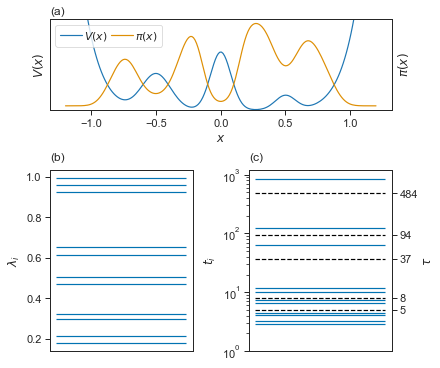
\includegraphics[width=0.8\textwidth]{chapters/hmm_selection/figures/prinz_pot.png}
    \label{fig:prinz}
\end{figure}


The Prinz potential \cite{prinzMarkovModelsMolecular2011} is a four well potential shown in figure \ref{fig:prinz}.  Panel (a) shows the potential, $V(x)$ in blue and the stationary distribution $\pi(x)$, with the four metastable states, in orange. From this potential  $100$ independent trajectories were sampled, discretised and used as data for estimating the HMMs in this work. See appendix \ref{app:hmm} for full details of the Prinz potential and simulation details. Panel (b) show the exact ratio of successive eigenvalues resolvable by a $\tau=5$ MSM. The large gap between the fourth and fifth eigenvalues is clearly seen, implying four metastable states. Panel (c) shows the exact ratio of implied timescales. The implied timescales show the largest gap between the second and third implied timescale. Panel (d) shows the mean implied timescales and \SI{95}{\percent} credible intervals as a function of the Markov lag time, estimated using these data with a Bayesian HMM. The exact timescales are shown as solid coloured lines. The number of hidden states was set was determined by the lag time and the exact timescales of the full Prinz transfer operator (see table \ref{tab:prinz_its_exact}). For example for $\tau = 130$ only $t_2 = 844$ is resolvable so a two hidden state HMM was used.

\subsubsection{AADH}
The data for the AADH system comprise the MSMs and associated discrete trajectories of the base case and three sensitivities described in chapter \ref{chap:msm} section \ref{subsubsec:sensitivity_analysis}. The model specifications are tabulated here in table \ref{tab:aadh_final_msm_specs}. 

\begin{table}
    \centering
    \mycaption{Markov lag time and MSM hyper-parameters. These MSMs and the associated discrete trajectories form the data for the HMM coarse graining.}
    \begin{tabular}{|l|l|l|l|l|}
        \hline
        Parameter & Base case & Sensitivity 1 & Sensitivity 2 & Sensitivity 3 \\
        \hline\hline
        Markov lag time, $\tau(\textrm{MSM})$ & \SI{2}{\nano\second} &  \SI{20}{\nano\second}& \SI{2}{\nano\second}& \SI{2}{\nano\second} \\
        Feature, $\chi$ & $(\phi, \psi, \chi)$ & $(\phi, \psi, \chi)$ & $|\mathbf{r}_{1}-\mathbf{r}_2|$ & $(\phi, \psi, \chi)$ \\
        TICA lag time, $\tau$ & \SI{10}{\nano\second} & \SI{10}{\nano\second}&\SI{1}{\nano\second} &\SI{85}{\nano\second} \\
        TICA components, $m$ & $2$ & $2$ & $2$ & $2$ \\
        Cluster centres, $n$ & $310$ & $310$ & $110$ & $310$ \\
        \hline
    \end{tabular}
    \label{tab:aadh_final_msm_specs}
\end{table}

\subsection{Model selection criteria}

This work will compare the use of the following model selection techniques for selecting the number of hidden states in a HMM: 
\begin{enumerate}
    \item The Akaike Information Criterion, AIC; 
    \item The cross-validated log-likelihood, CVLL; 
    \item The Bayesian Information Criterion, BIC; 
    \item The Integrated Classification Likelihood Criterion, ICL.
\end{enumerate}

Each of these will be defined in the sections that follow but a number of common concepts and conventions are useful to define first. 

The likelihood of  a hidden Markov model is given by \cite{noeProjectedHiddenMarkov2013a}: 
\begin{equation}\label{eqn:obs_lik_full}
\begin{split}
    L(\tilde{\mathbf{T}}, \mathbf{E}; \{s_t\}) & = p(\{s_t\} | \tilde{\mathbf{T}}, \mathbf{E}) \\
    & = \sum_{\substack{\{h_t\} \in \\ \text{all paths}}} \tilde{\pi}E_{s_{0}, h_{0}}\prod_{t=1}^{t_{max}}\tilde{T}_{h_{t-1}, h_t}E_{s_t, h_t}    
\end{split}
\end{equation}


Here $\{s_t\}$ are the observed state trajectories and $\{h_t\}$ are the (unknown) hidden state trajectories. This quantity will be simplified to $L(\theta)$. likelihood is maximized by the Baum Welch algorithm [][] and the corresponding value will be denoted $L(\hat{\theta})$ where $\hat{\theta}$ are the maximum likelihood estimates of the HMM parameters. It is usual to work with the log likelihood and this will be denoted $LL(\hat{\theta})$. 

The optimal values of the CVLL and the AIC both minimize the \emph{Kullback-Leibler} divergence, $D_{KL}(p||p^*)$ - a measure of the difference of one probability distribution, here the modelled distribution,  $p(\{s_t\} | \hat{\theta})$  and a reference distribution, $p^{*}(\{s_t\})$: 

\begin{equation}\label{eqn:kl_div}
\begin{split}
    D_{KL}(p||p^*) & = \int p^{*}(\{s_t\}) \log{\left(\frac{ p^{*}(\{s_t\}) }{p(\{s_t\} | \hat{\theta})}  \right)} d(\{s_t\}) \\ 
    & = \int p^{*}(\{s_t\}) \log{\left(p^{*}(\{s_t\})\right)}d(\{s_t\}) - \int p^{*}(\{s_t\})\log{\left(p(\{s_t\} | \hat{\theta})\right)} d(\{s_t\})
\end{split}
\end{equation}

The optimal values of the BIC and ICL maximize the types of integrated likelihood. Minimizing the BIC is equivalent to choosing the model with the largest Bayes factor or the model with the largest posterior probability, given the data. The likelihood used is the observed likelihood (equation \ref{eqn:obs_lik_full}) but integrated over the parameters $\tilde{\mathbf{T}}$ and $\mathbf{E}$: 

\begin{equation}\label{eqn:obs_lik_int}
        p(\{s_t\}) = \int p\left(\{s_{t}\}\middle |\theta \right)p(\theta) \mathrm{d}\theta
\end{equation}

In the case of the ICL, the likelihood is the complete data likelihood: 
\begin{equation}\label{eqn:class_lik_int}
    p(\{(s_t, h_t)\} = \int p\left(\{(s_{t}, h_{t})\}\middle |\theta \right)p(\theta) \mathrm{d}\theta
\end{equation}

Although the hidden states are not observed, the hidden states for each MD frame is  taken to be the state with the largest posterior probability, given the observed state i.e. $\arg\max_{i}p(h=i|s=j)$.  


\subsubsection{The Akaike Information Criterion, AIC}. 

The AIC is defined as:
\begin{equation}\label{eqn:aic}
    \operatorname{AIC} = -2\left(\log{L\left(\{s_t\}|\hat{\theta}\right)} - d\right)
\end{equation}
where $d$ is the number of degrees of freedom of the model. For a reversible hidden Markov model with $g$ hidden states and $n$ observed states  $d = \sfrac{1}{2}g(g-1) + (g-1) + g(n-1)$ \cite{trendelkamp-schroerEstimationUncertaintyReversible2015b}. 


The AIC arises from the approximation of the second term in the definition of the $D_{KL}$ (equation \ref{eqn:kl_div}), the first being independent of the model and thus irrelevant. The derivation starts by approximating the true distribution $p^{*}(\{s_t\})$ with the empirical distribution, giving rise to the $\log{L\left(\{s_t\}|\hat{\theta}\right)}$ term.  This will naturally over-fit to the data and the  $d$ term is a bias correction term to account for this.  $d$ is only equal to the degrees of freedom of the model under the assumption that the true model is under consideration. The $-2$ is there to make an equivalence with Mallows $C_p$ \cite{friedman2001elements}. The selected model is the one which has the smallest AIC or in other words, the model which has the smallest KL divergence relative to the true data generating process. 

\subsubsection{The cross-validated log-likelihood, CVLL}. Maximizing the the cross-validated log-likelihood also minimizes the KL-divergence \cite{celeuxSelectingHiddenMarkov2008}. The CVLL is calculated in the following way: 
\begin{enumerate}
    \item The observed trajectories are split into $N$ training $\{s_t\}^{i}$ and test $\{s_t\}^{-i}$, $i = 1, ..., N$ sets using 50:50 shuffle-split, as described in chapter \ref{chap:msm} section \ref{sec:methods}. 
    \item For each $i$, fit a HMM using the training data $\{s_t\}^{i}$. 
    \item Calculate the likelihood using the test data,  $L(\hat{\theta}^{i}|\{s_t\}^{-i})$, using the forward part of the Baum-Welch algorithm. 
    \item The Cross-validated log-likelihood is then average over the splits: 
    \begin{equation}
        \operatorname{CVLL} = \frac{1}{N}\sum_{i}^{N}L\left(\theta \middle |\{s\}^{-i}\right)
    \end{equation}
\end{enumerate}

In order to make the values of the CVLL comparable to the other criteria the CVLL was multiplied by: $2$ to account for the parameters being estimated on half of the data (and the log-likelihood scales linearly with the number of observations), and then $-2$ to account for the same factor in the definition of AIC, BIC and ICL. Thus the \emph{minimum} of the CVLL determines the selected model.  


\subsubsection{Bayesian information criterion, BIC}. 

The BIC is defined as: 
\begin{equation}\label{eqn:bic}
    \operatorname{BIC} = -2\left(\log{\left(L\left(\{s_t\}\middle|\theta\right)\right)} - \frac{1}{2}d\log{\left(N_{obs}\right)}\right)
\end{equation}
where $d$ is the degrees of freedom and $N_{obs}$ is the number of observations.  The difference in BIC between two models, $BIC_{1}-BIC_{2}$ is an approximation to the log of the Bayes factor, the selected model is then the one with the smallest BIC. The number of observations is equal to the number of pairs of frames separated by the lag time and so decreases with $\tau$. If there are $q$ independent MD trajectories, of $t_{max}$ frames each, then the number of observations is $N_{obs} = q(t_{max}-\tau)$. The derivation of the BIC approximates the log of the observed likelihood,  $\log{\left(p(\{s_t\}\right)}$, (see equation \ref{eqn:obs_lik_int}) under the assumption that the prior distribution of the parameters $p(\theta)$ is relatively non-informative. There are several drawbacks to the use of the BIC in assessing the number of components in mixture models. First like the AIC, the BIC is also only valid under the assumption that the true model is in the models under consideration. Second,  use of the BIC for assessing mixture models  is not theoretically justified, however simulation studies have shown it to be useful [].  

\subsubsection{Integrated classification likelihood criterion, ICL}. 
The integrated classification likelihood criterion is derived in a  similar fashion to the BIC, but the starting point is the classification likelihood, equation \ref{eqn:class_lik_int}. The final approximation to $\log{(p(\{(s_t, h_t)\})}$ becomes: 

\begin{equation}\label{eqn:icl}
\begin{split}
        \operatorname{ICL} &= -2\left(\log{\left(L\left(\{(s_t, h_{t})\}\middle|\theta\right)\right)} - H\left(\mathbf{M}\right) - \frac{1}{2}d\log{\left(N_{obs}\right)}\right)     \\
        & = \operatorname{BIC} + 2H\left(\mathbf{M}\right)
\end{split}
\end{equation}

The $H\left(\mathbf{M}\right)$ is classification entropy, it is  the information entropy for assignment of each observation to a hidden state, summed over all the observations: 
\begin{equation}
    H(\mathbf{M}) = -\sum_{t}^{t_{max}} \sum_{j}^{g} M_{s_{t}, j}\log{\left(M_{s_{t}, j}\right)}
\end{equation}

The elements of the membership matrix  $M_{i,j}$ are the probability of being in a hidden state $j$ given an observed state $i$, $P(h=j|s=i)$. The inner sum is the entropy of single observation which quantifies the uncertainty with which the model assigns the given observed state to a hidden state. For example in a two hidden state system the classification entropy for a single observed state $i$ will be $p(h=1|s_t=i)\log{p(h=1|s_t=i)} + p(h=2|s_t=i)\log{p(h=2|s_t=i)}$. The ICL inherits the drawbacks and assumptions of the BIC but has been shown to be practically useful for selecting the number of components in mixture models. 


\subsection{Model selection}

The model selection criteria, CVLL, AIC, BIC and ICL, will be used to select the optimum number of hidden states in a maximum likelihood HMM, using the discrete trajectories sampled from the Prinz potential. Five different values of the Markov lag time will be used, they are $\tau=5, 8, 15, 65, 130$. These values of $\tau$ were chosen because they resolve, respectively $7, 5, 3, 2, 1$ implied timescales in the full MSM state space. As the top three of these timescales are dominant, they resolve $4, 4, 4, 3, 2$ hidden states and so provide an easy way of comparing the performance of the indicators over different numbers of true hidden states\cite{noeProjectedHiddenMarkov2013a}. The implied timescales for HMMs using the `true' number of states is shown in figure \ref{fig:prinz}, panel (b). The vertical black lines are located at the chosen values of $\tau$.

For each value of $\tau$, nine different maximum likelihood Markov models were estimated with $2 - 10$ hidden states. Up to four different models were selected by the four selection criteria and these were compared to the model with the true number of hidden states by means of the Chapman-Kolmogorov test using Bayesian estimation to determine the uncertainty in the parameter estimates. However, the CK test was only performed if a Bayesian model could be converged. The convergence criterion was set to $|\hat{R}-1|<0.1$ using Gelman-Rubin R-hat statistic on two independent MCMC chains. The same methodology was applied to the four different discretisations and values of $\tau$ tabulated in table \ref{tab:aadh_final_msm_specs}. 


\section{Results and discussion}\label{sec:hmm_results}
\subsection{Prinz Potential}

\begin{table}
    \centering
    \mycaption{The selected number of hidden states, $\hat{g}$, by the CVLL, AIC, BIC and ICL for each value of $\tau$. The true values, $g^{\mathrm{true}}$ are also shown. Numbers highlighted in bold are where $\hat{g}=g^{\mathrm{true}}$. }
    \begin{tabular}{|c|c|c|c|c|c|}
    \hline
    $\tau$ & $g^{\mathrm{true}}$ & CVLL & AIC & BIC & ICL  \\
    \hline\hline
     $5$  & $4$ & $\mathbf{4}$  & $10$ & $10$ & $5$ \\
     $8$  & $4$ & $\mathbf{4}$ & $10$ & $8$  & $\mathbf{4}$  \\
     $15$ & $4$ & $\mathbf{4}$  & $9$  & $6$  & $\mathbf{4}$  \\
     $65 $& $3$ & $4$  & $5$  & $4$  & $\mathbf{3}$  \\
     $130$& $2$ & $4$  & $4$  & $3$  & $3$  \\
     \hline
    \end{tabular}
    \label{tab:prinz_criteria_results}
\end{table}

The selected number of hidden states using each criterion are shown in table \ref{tab:prinz_criteria_results}.  The ICL performs best by correctly identifying the number of hidden states in three out of the five different cases. 
It fails at $\tau=5$ where the estimated implied timescales (figure \ref{fig:prinz}, panel (d)) show the model is not quite Markovian. The selected value of $5$ is close to the true value of $4$  and the relative values of the ICL for $g=4 - 7$ are also quite similar with less than \SI{1}{\percent} difference between them, see figure \ref{fig:prinz_criteria_results} panel (a)(iv). It also fails at $\tau=130$, however the relative values for the selected and true value are similar (less than \SI{1}{\percent} difference), while for $g>3$ the value of the ICL increases rapidly, see panel (e)(iv). The cross-validated log likelihood also correctly predicts four states, however 

In all other cases the number of hidden states is over-estimated. This is inline with previous simulation studies of these criteria [][][]. The BIC performs best out of the other criteria, only over-estimating the number of states by $1$ for $\tau=65, 130$. 

\begin{figure}
    \centering
    \mycaption{Hidden state selection criteria for HMMs with $\tau=5, 8, 15, 65, 130$, rows (a) - (e). The best performing number of hidden states is indicated by an arrow. Column (i) shows the cross-validated log-likelihood ($\operatorname{CVLL}$). Column (ii) shows the AIC. The log-likelihood term is shown in blue and the degrees of freedom penalty ($2d$) is shown in orange. Column (iii) shows the BIC. The penalty term $d\cdot\log{N}$ is shown in green.  Column (iv) shows ICL. The classification entropy penalty term $2\cdot H$ is shown in red. Missing values indicate the failure of the HMM to converge. All values have been scaled so the minimum value in each panel is $1$.}
    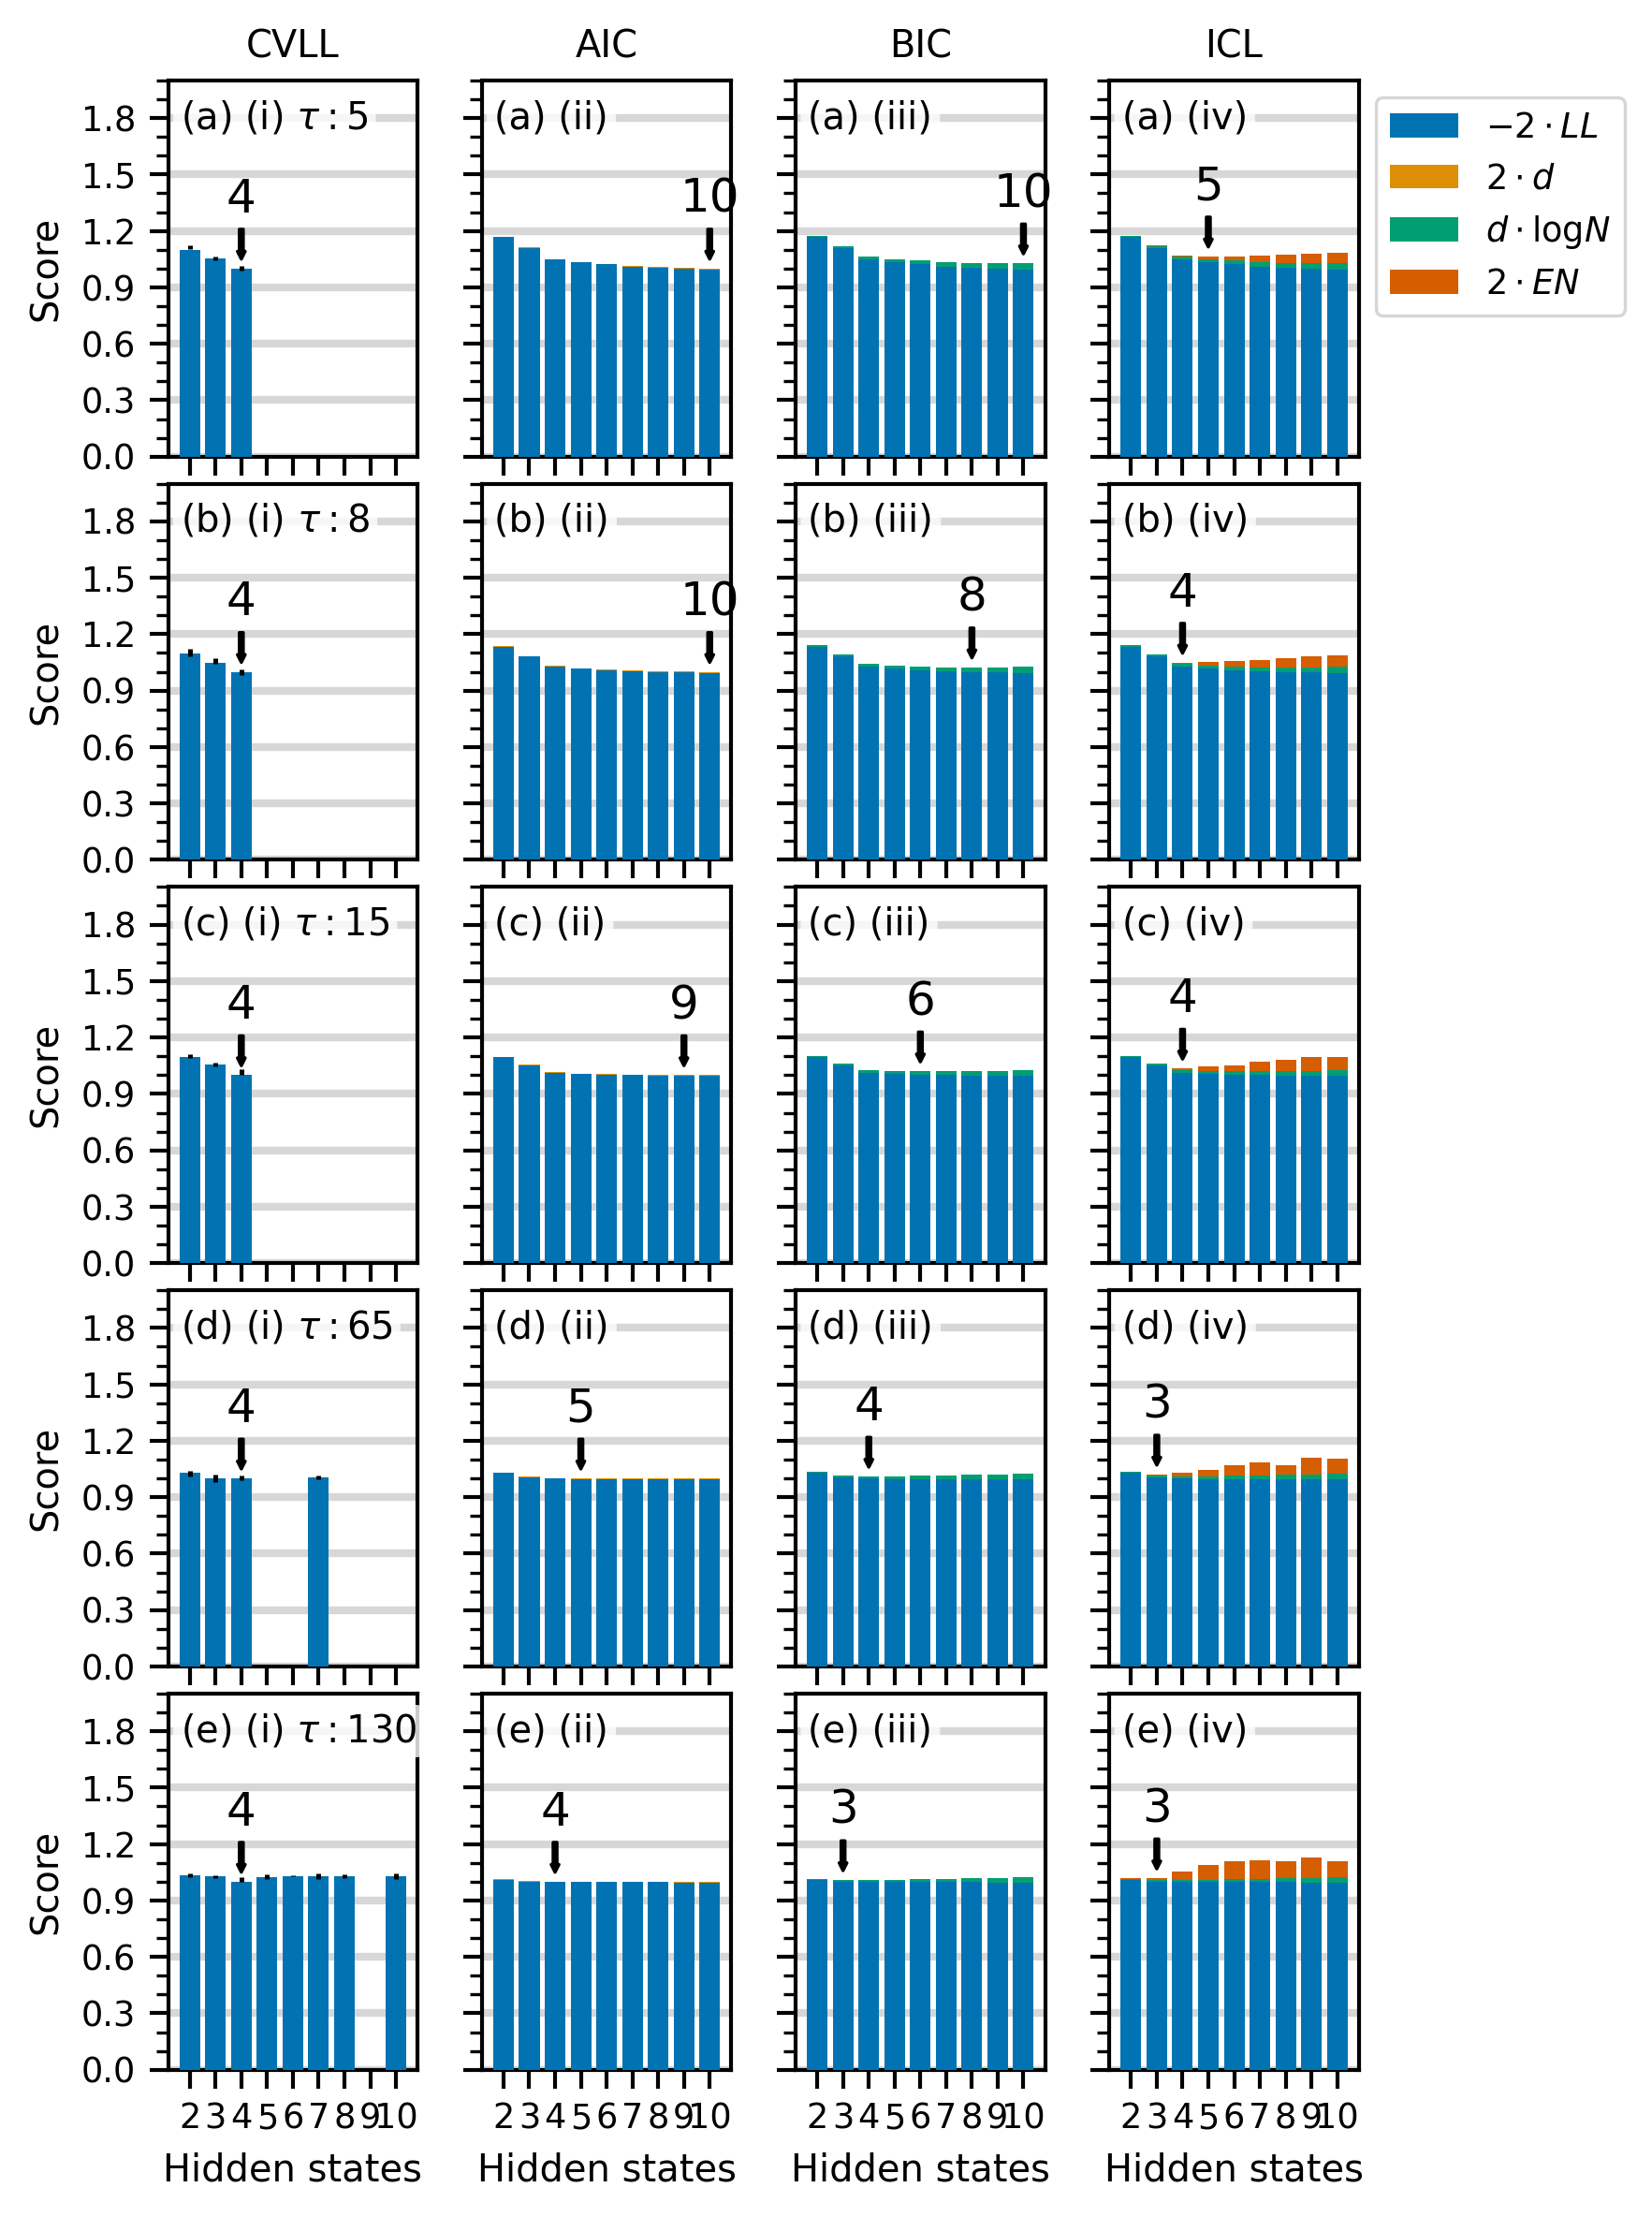
\includegraphics[width=0.75\textwidth]{chapters/hmm_selection/figures/prinz_h_state_selection.png}
    \label{fig:prinz_criteria_results}
\end{figure}

The relative values of the selection criteria are shown in figure \ref{fig:prinz_criteria_results}. Each row, (a) - (e), corresponds to a different value of the Markov lag time $\tau=5, 8, 15, 65, 130$. Each column, (i) - (iv), corresponds to the different model selection criteria, CVLL, AIC, BIC, and ICL. The minimum value of each criteria for each model is highlighted with an arrow indicating the estimated number of hidden states, $\hat{g}$. The values are scaled so the value at the selected number of states is equal to $1$.  The coloured bars show the contributions of the different parts of each score. The blue bars shows the log-likelihood terms of equations \ref{eqn:aic}, \ref{eqn:bic} and \ref{eqn:icl} i.e.  $-2\times LL$. In the case of CVLL, the blue bars are the  cross-validated equivalent. The various penalty terms are shown in orange ($2d$ the AIC penalty), green ($d\log{N}$, the BIC penalty) and red ($2H(\mathbf{M})$, the classification entropy).  

The cross-validated log-likelihood, CVLL, (and the log-likelihood),  is invariant to the number of hidden states for large $\tau$ but increase markedly for small $\tau$.  Small values of $\tau$ enables resolution of the fast relaxation processes (within a potential well for example) and for these to be captured in the HMM transition matrix. So even though the number of states is high from the point of view of clustering the state space into distinct metastable states, the high number of states is still able to capture the 

For large $\tau$ these fast relaxation processes cannot be captured and so estimation using large numbers of states results in noisy estimates of the parameters. 

In the case of log-likelihood, increase in log-likelihood is perfectly monotonic and the AIC selected models with $g < 10$ is due to the over-fitting penalty $2d$.

the trend of favouring  we would expect this trend to continue for increasing $g$ as the number of hidden states fits to spurious 


Points to note: 
\begin{enumerate}
    \item The Chapman-Kolmogorov tests do not differentiate between $g = 2, 3, 4$ states up to $10\tau$ I.e. $T(\tau)^10 = T(10\tau)$ for $g = 2, 3, 4$ hidden states. See figures \ref{fig:prinz_ck_test_5_2} to \ref{fig:prinz_ck_test_5_4}. There's only four states for $\tau < 64$ (the third relaxation process has a lifetime of $64$ time steps. 
    \item There is a cross-validated log likelihood difference between $g = 2 - 4$, see figure \ref{fig:prinz_criteria_results} panel (a)(i) (and for that matter, the non-cross-validated log-likelihood (a)(ii) blue bars) which favours $4$ vs $3,2$. 
    \item However, the likelihood criteria overestimate the number of hidden states. The closest is the ICL with $g=5$. The CK tests for $g=5, 9, 10$ are shown in figures \ref{fig:prinz_ck_test_5_5} - \ref{fig:prinz_ck_test_5_10}. They are re-assuringly rubbish. 
    \item Contra the Noe HMM paper \cite{noeProjectedHiddenMarkov2013a}, increasing the number of hidden states above the `actual' number i.e. $g = 5, 6, 7, 8, 9$, doesn't affect the timescale estimates of the `true' timescales, see figure \ref{fig:prinz_its_tau_5}.
    \item it's puzzling that the likelihood increases for increasing $g$, even the cross-validated value. The likely reason has to do with that the hidden states for $g = 9$ (for instance) overlap a lot. See the lhs panes in figure \ref{fig:prinz_emission_dens_tau_5}.  
\end{enumerate}


\begin{figure}
    \centering
    \caption{The emission matrices for HMMs with g = $2, 3, 4, 5 9, 10$ hidden states}
    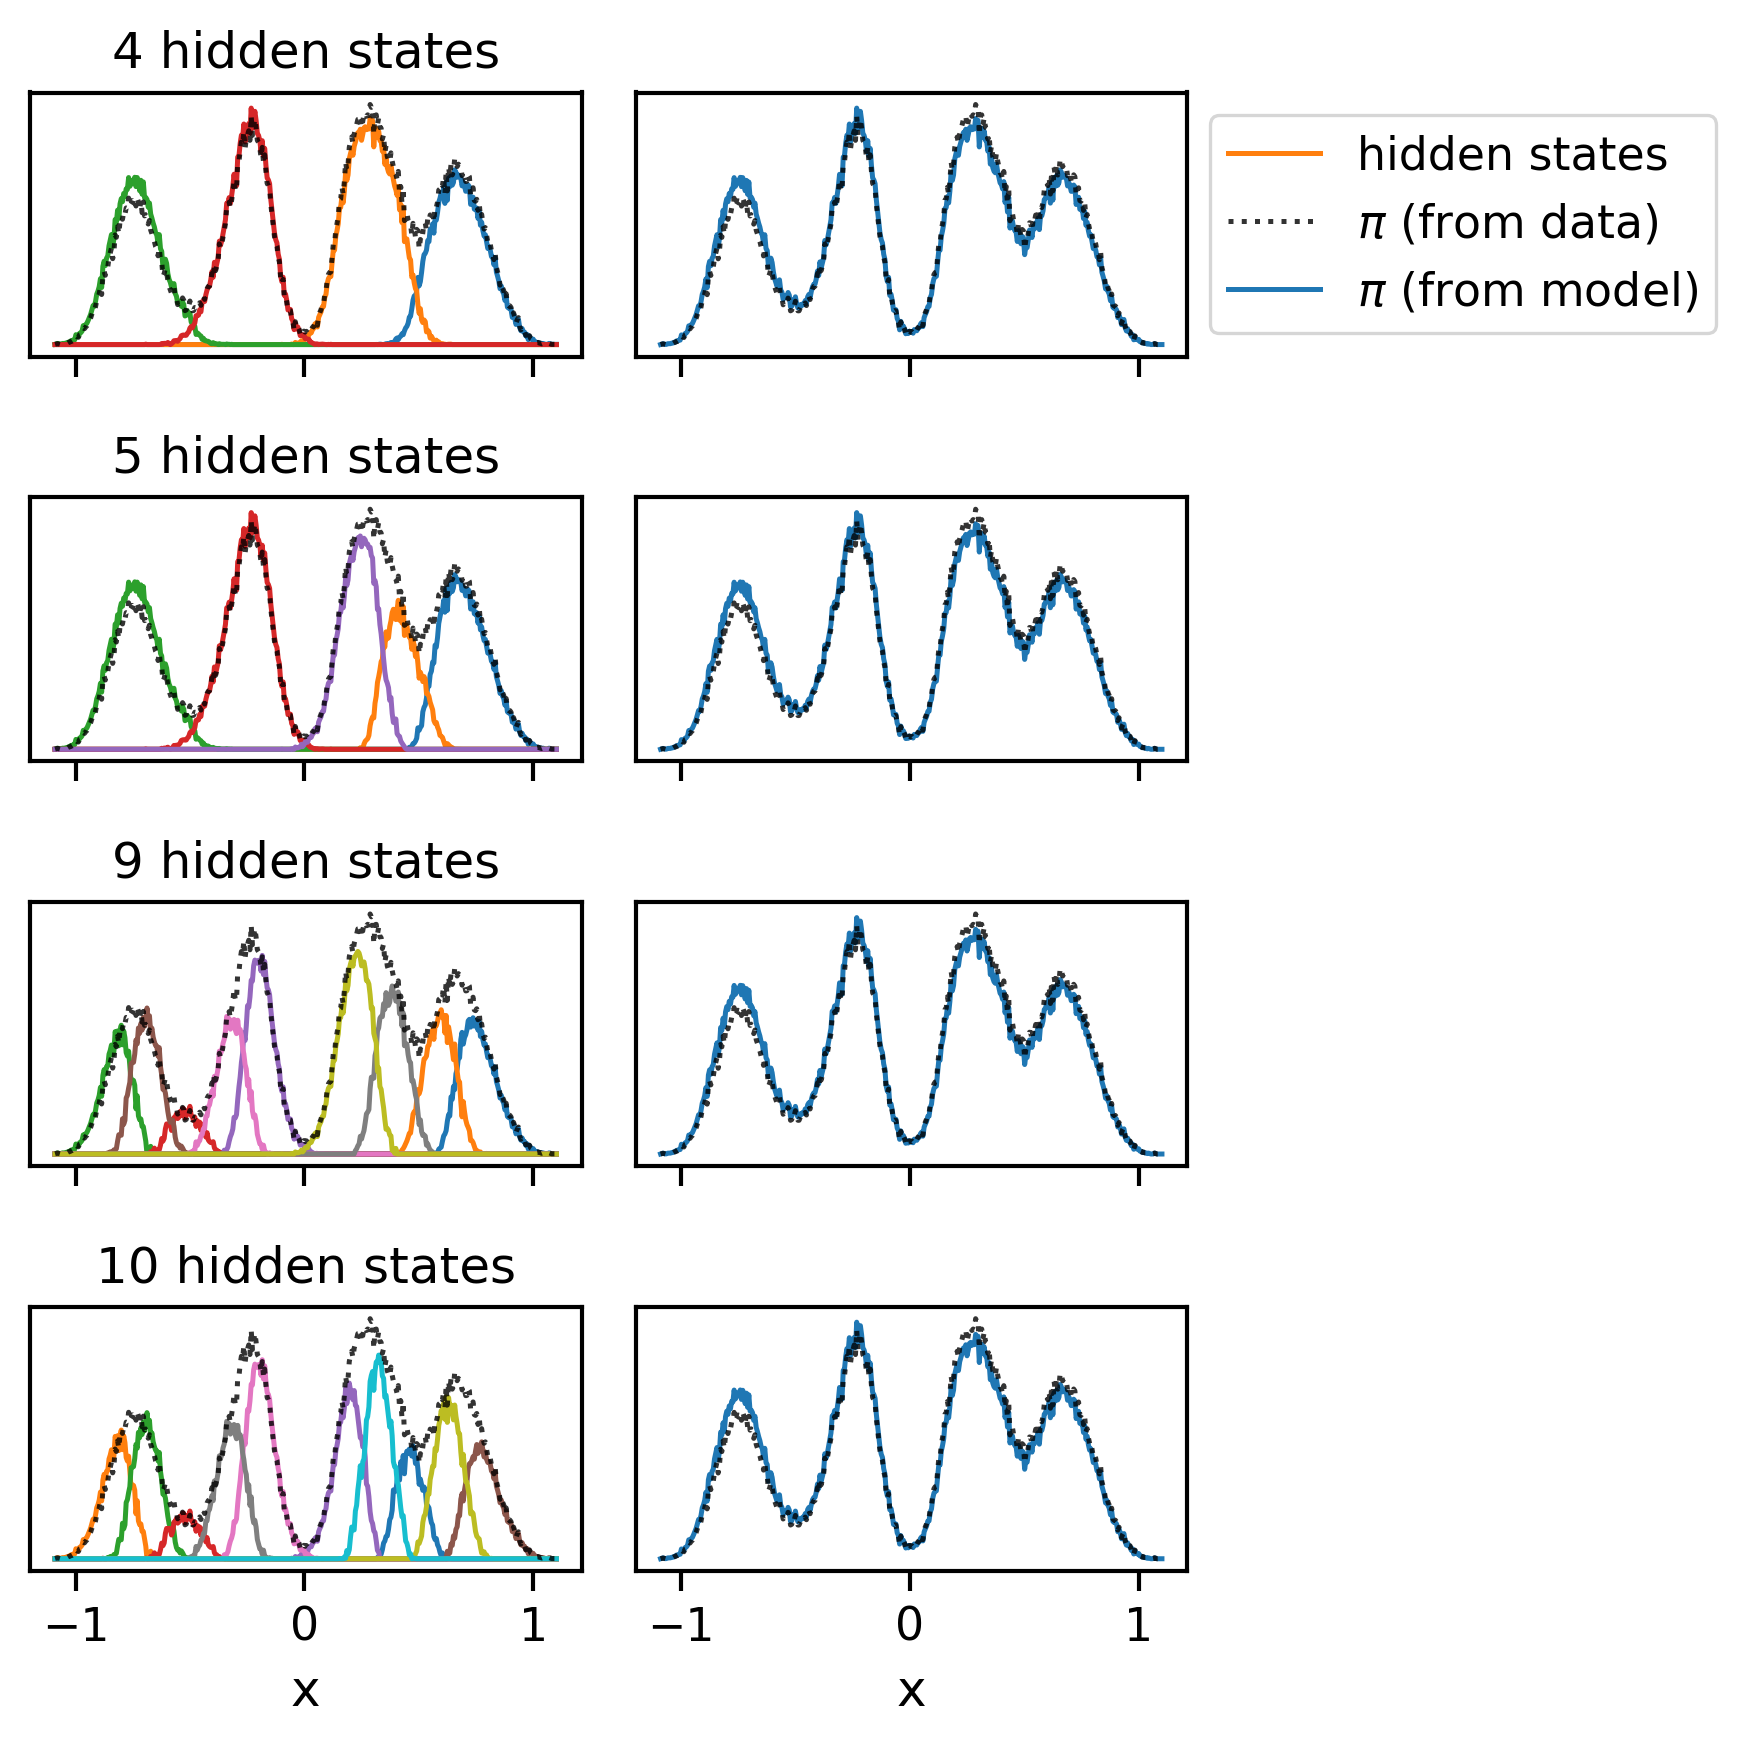
\includegraphics{chapters/hmm_selection/figures/prinz_emitted_densities_tau_5.png}
    \label{fig:prinz_emission_dens_tau_5}
\end{figure}






% A tentative explanation is as follows. The full expression for the observed likelihood for a trajectory of $t$ MD frames is
% \cite{noeProjectedHiddenMarkov2013a}: 

% \begin{equation}
% \mathbb{P}\left(\left\{s_{t}\right\} \mid \tilde{\mathbf{T}}, \mathbf{E}\right)=\sum_{\text {hidden paths }} \tilde{\pi}_{h_{0}} \mathbf{E}_{s_{0} h_{0}} \prod_{t=1}^{t_{\max }} \tilde{T}_{h_{t-1} h_{t}} \mathbf{E}_{s_{t} h_{t}},
% \end{equation}

% with initial distribution $\tilde{\pi}_{h_{0}}$ is approximated by the stationary distribution, $\tilde{\pi}$.  For each hidden path, i.e. the sequence of hidden states for each frame of the MD trajectory, the likelihood is comprised of the $t$ products of the probability of transitioning into a hidden state $h_j$, and the conditional probability of observing a state $s_i$ given the hidden state. 
% [More explanation]




\subsection{AADH}

\section{Conclusions}


% \begin{figure}
%     \centering
%     \begin{minipage}{0.4\textwidth}
%         \centering 
%          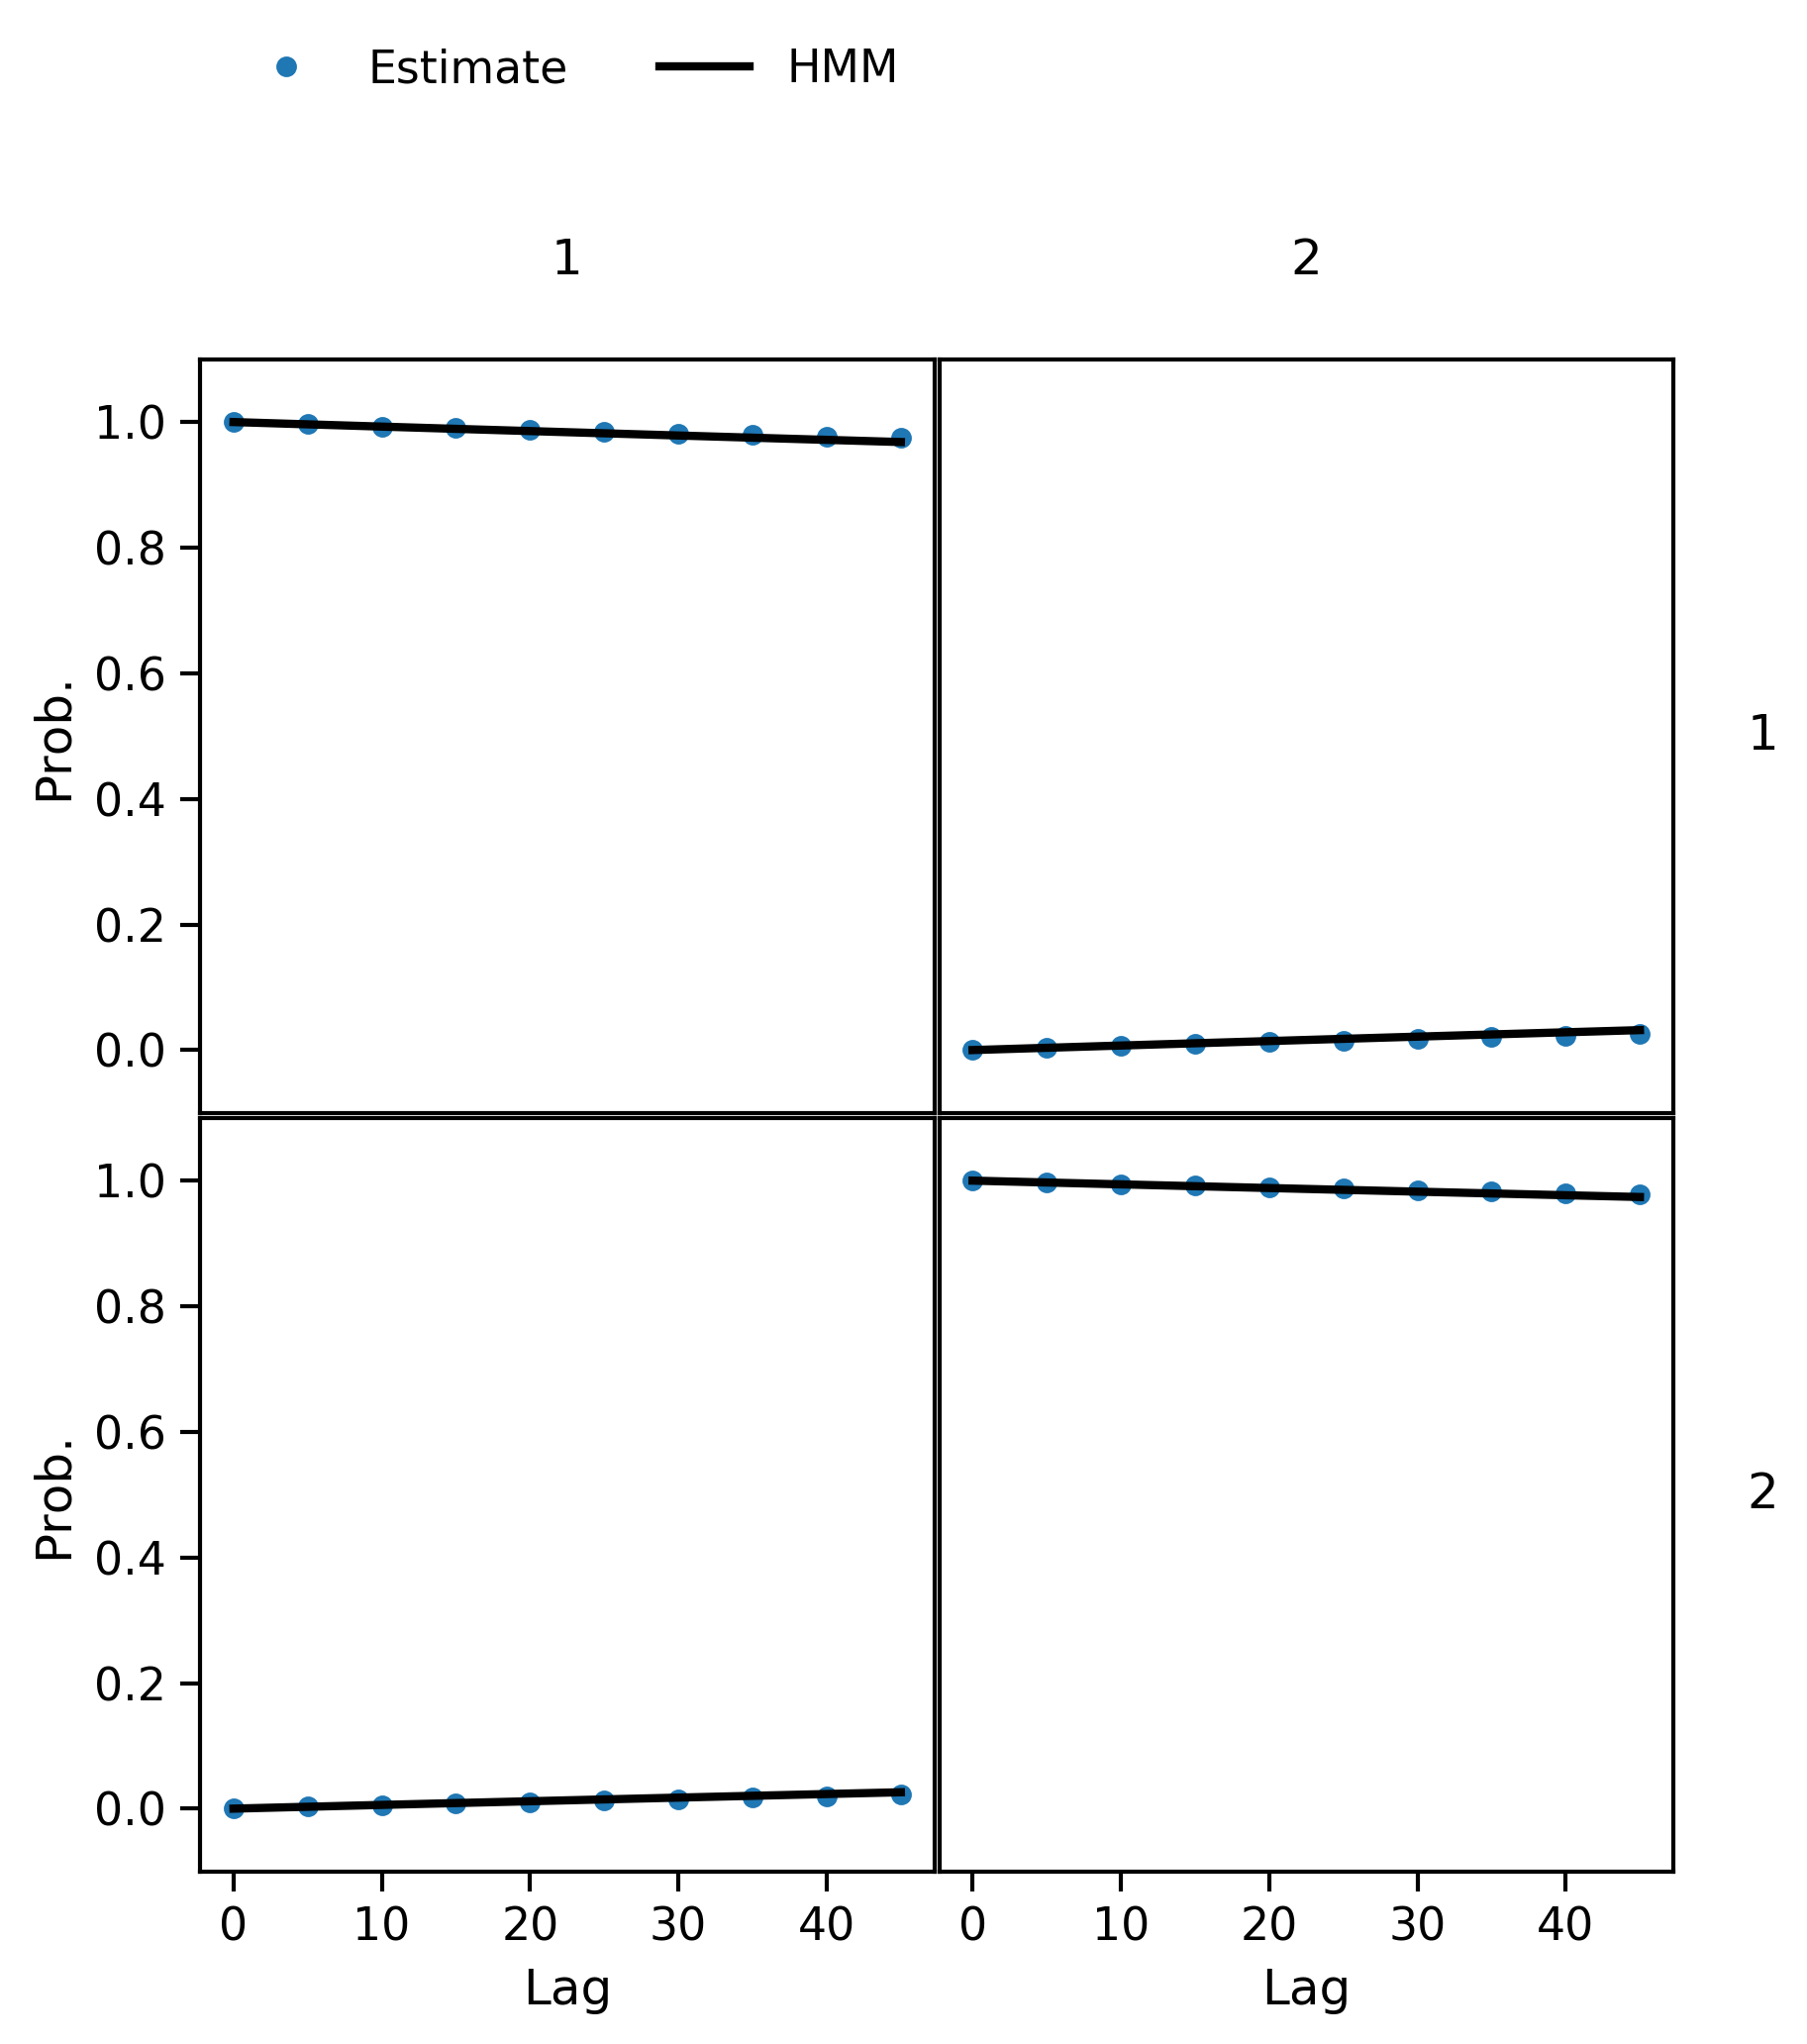
\includegraphics[width=0.8\linewidth]{chapters/hmm_selection/figures/ck_test_5_2.png}
%         \caption{CK test for Prinz Potential with $\tau=5$ and $g=2$} \label{fig:prinz_ck_test_5_2}
%     \end{minipage}
%     \hfill
%     \begin{minipage}{0.4\textwidth}
%         \centering
%          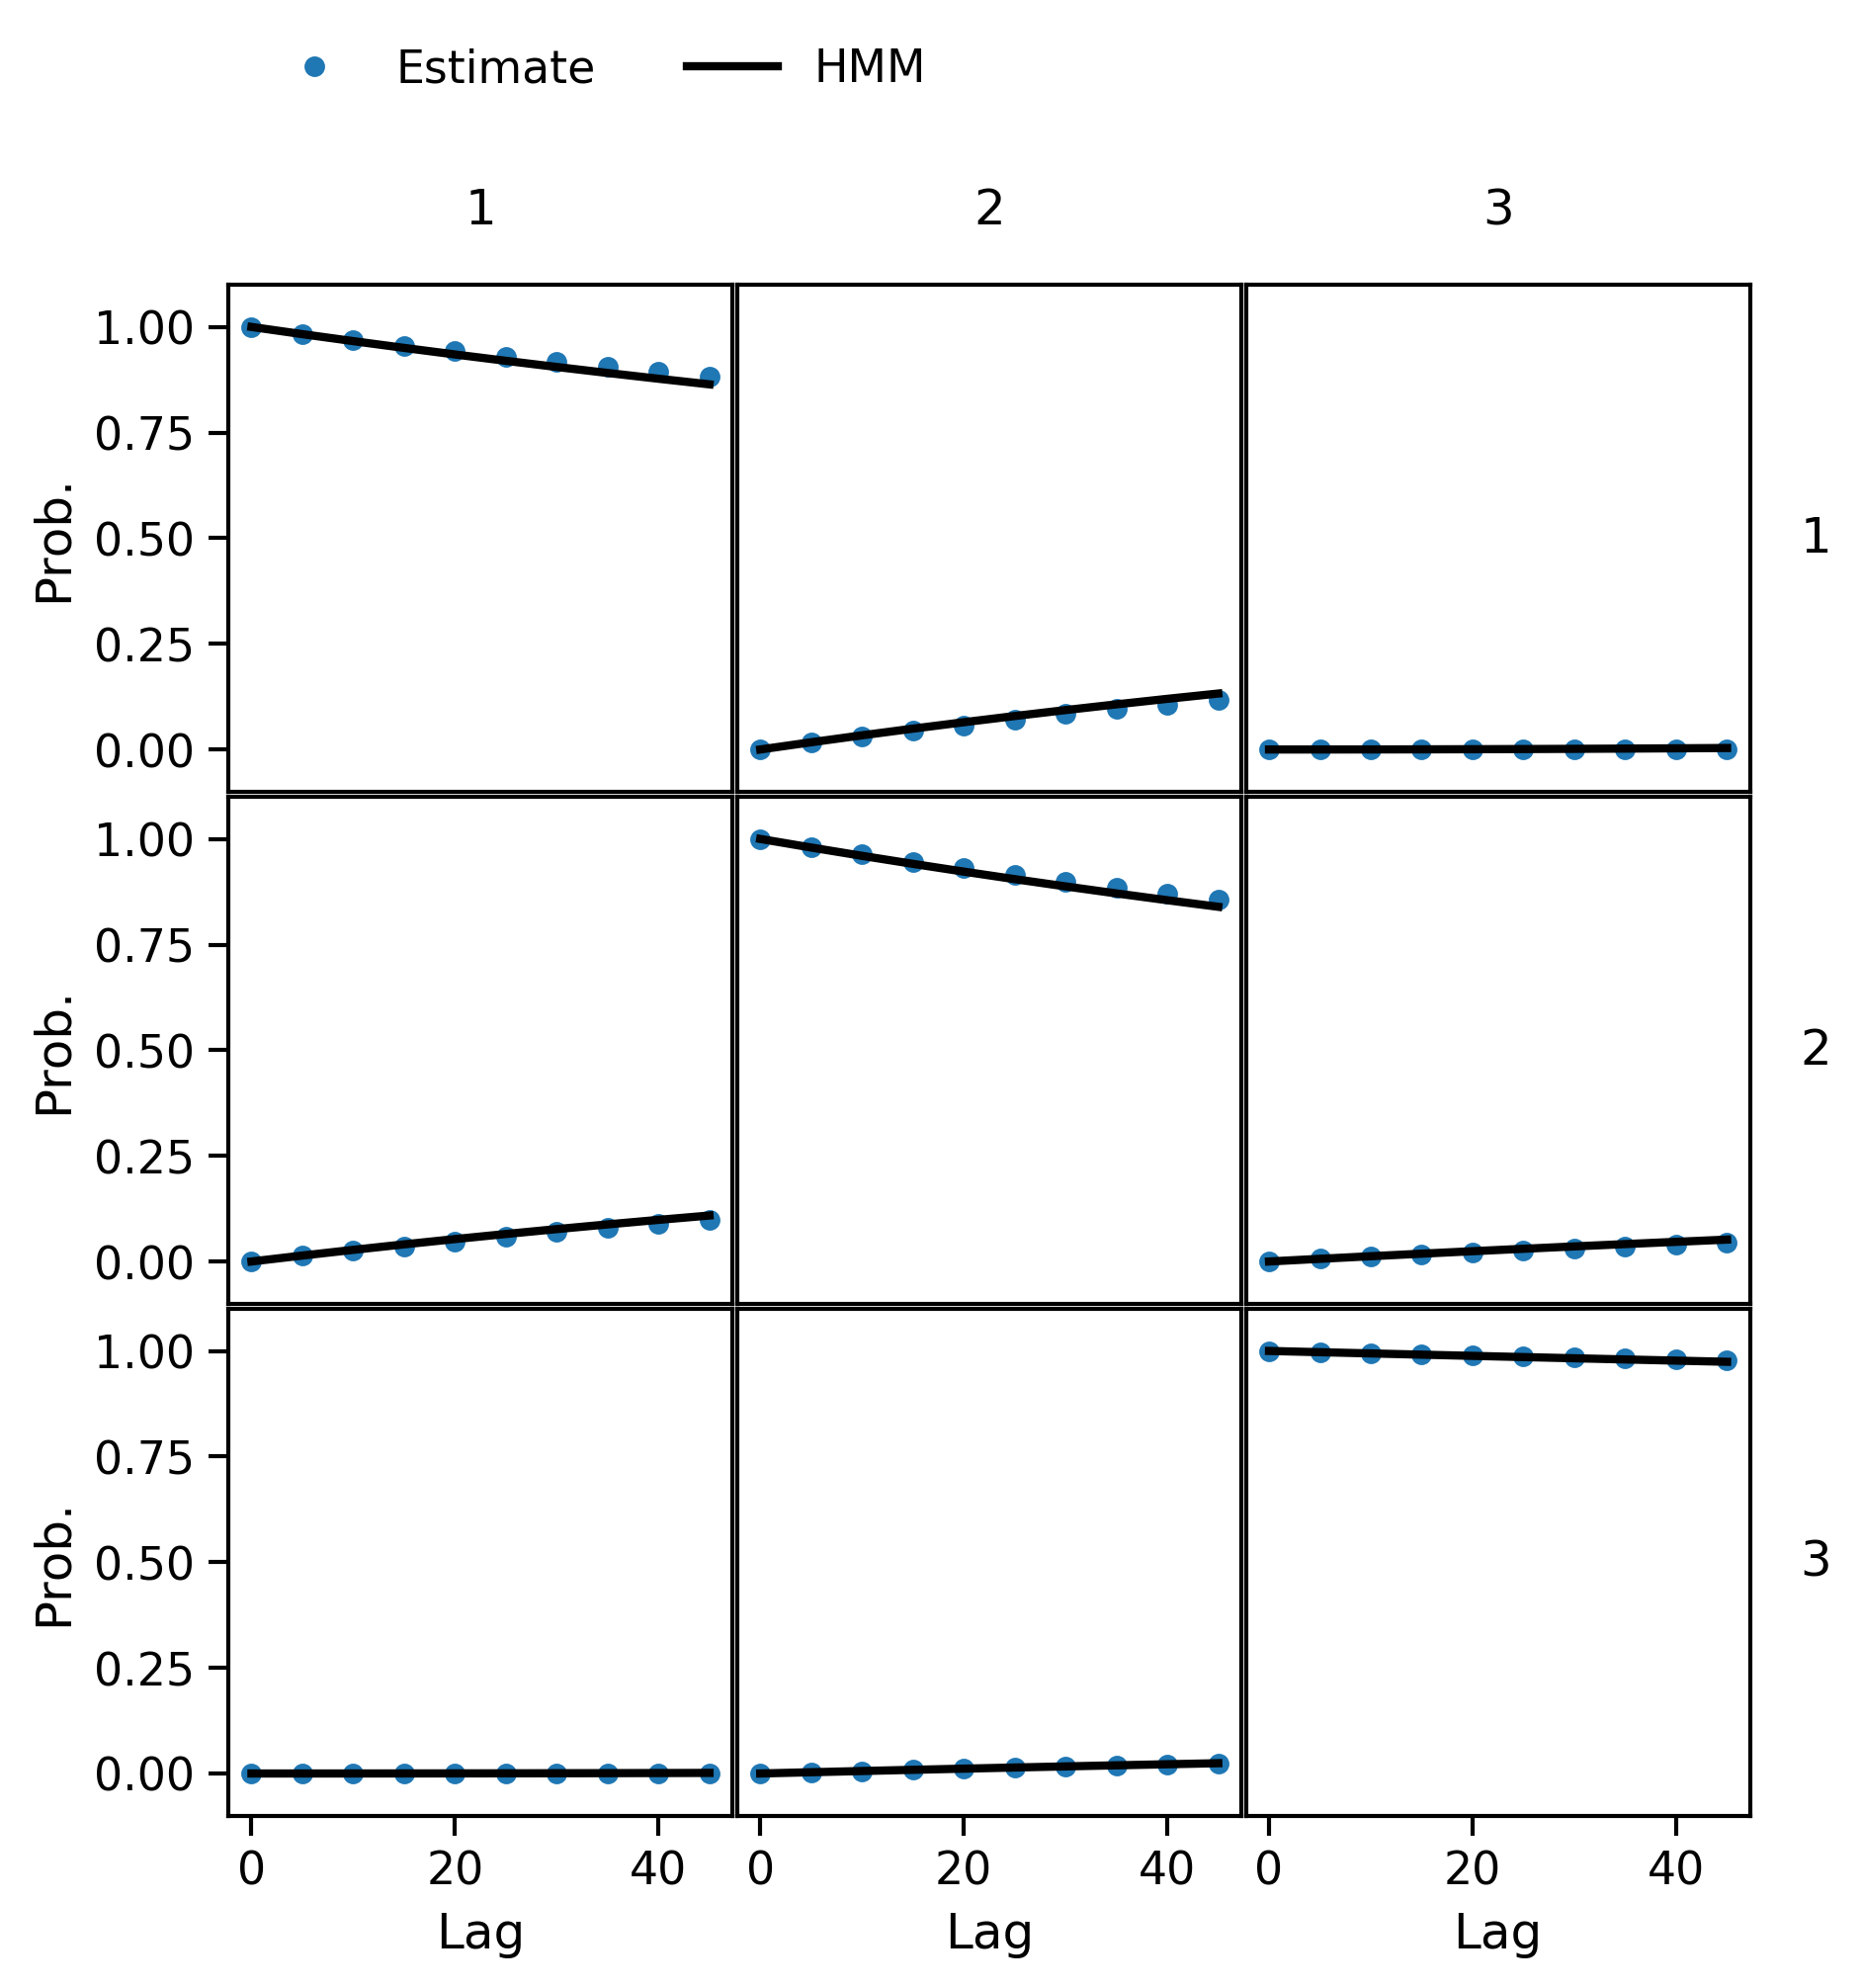
\includegraphics[width=0.8\linewidth]{chapters/hmm_selection/figures/ck_test_5_3.png}
%         \caption{CK test for Prinz Potential with $\tau=5$ and $g=3$} \label{fig:prinz_ck_test_5_3}
%     \end{minipage}
% \end{figure}



% \begin{figure}[p]
%     \centering
%     \mycaption{CK tests for Prinz Potential with $\tau = 5$ and $g = 2, 3$}
%     \subtop[$g = 2$]{
%         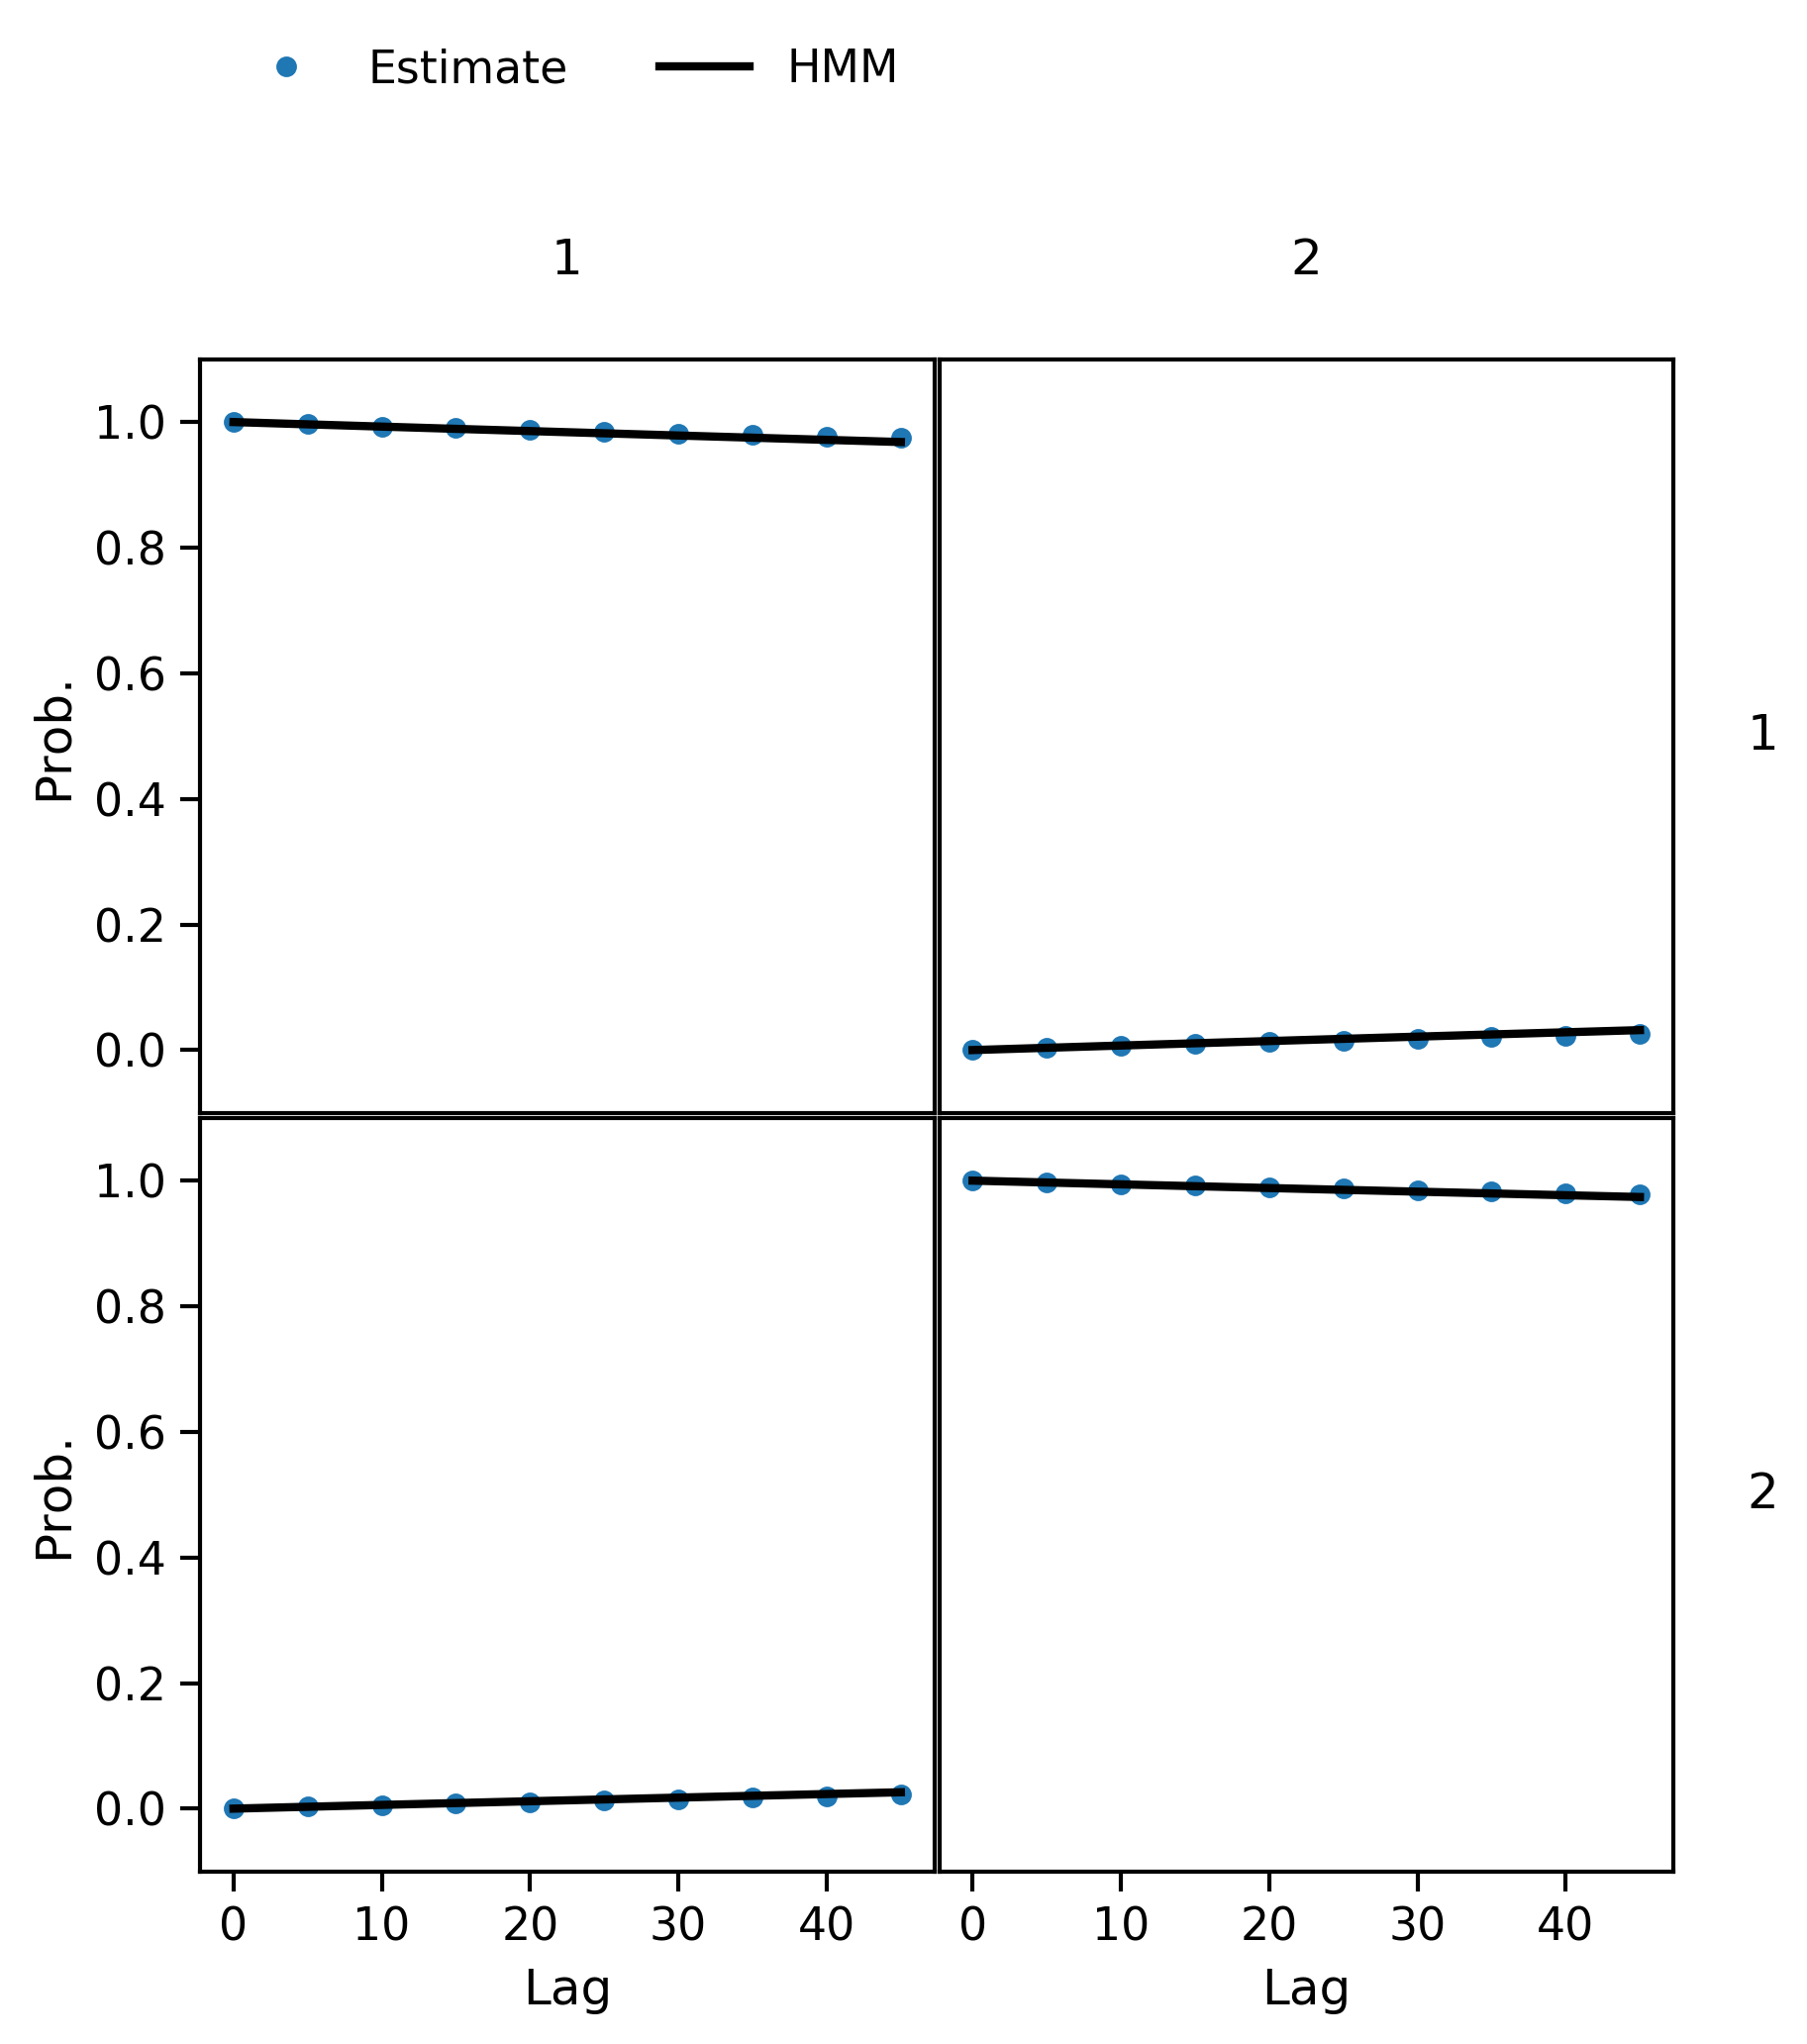
\includegraphics[width=0.4\textwidth]{chapters/hmm_selection/figures/ck_test_5_2.png}}
    
%     \subtop[$g = 3$]{
%         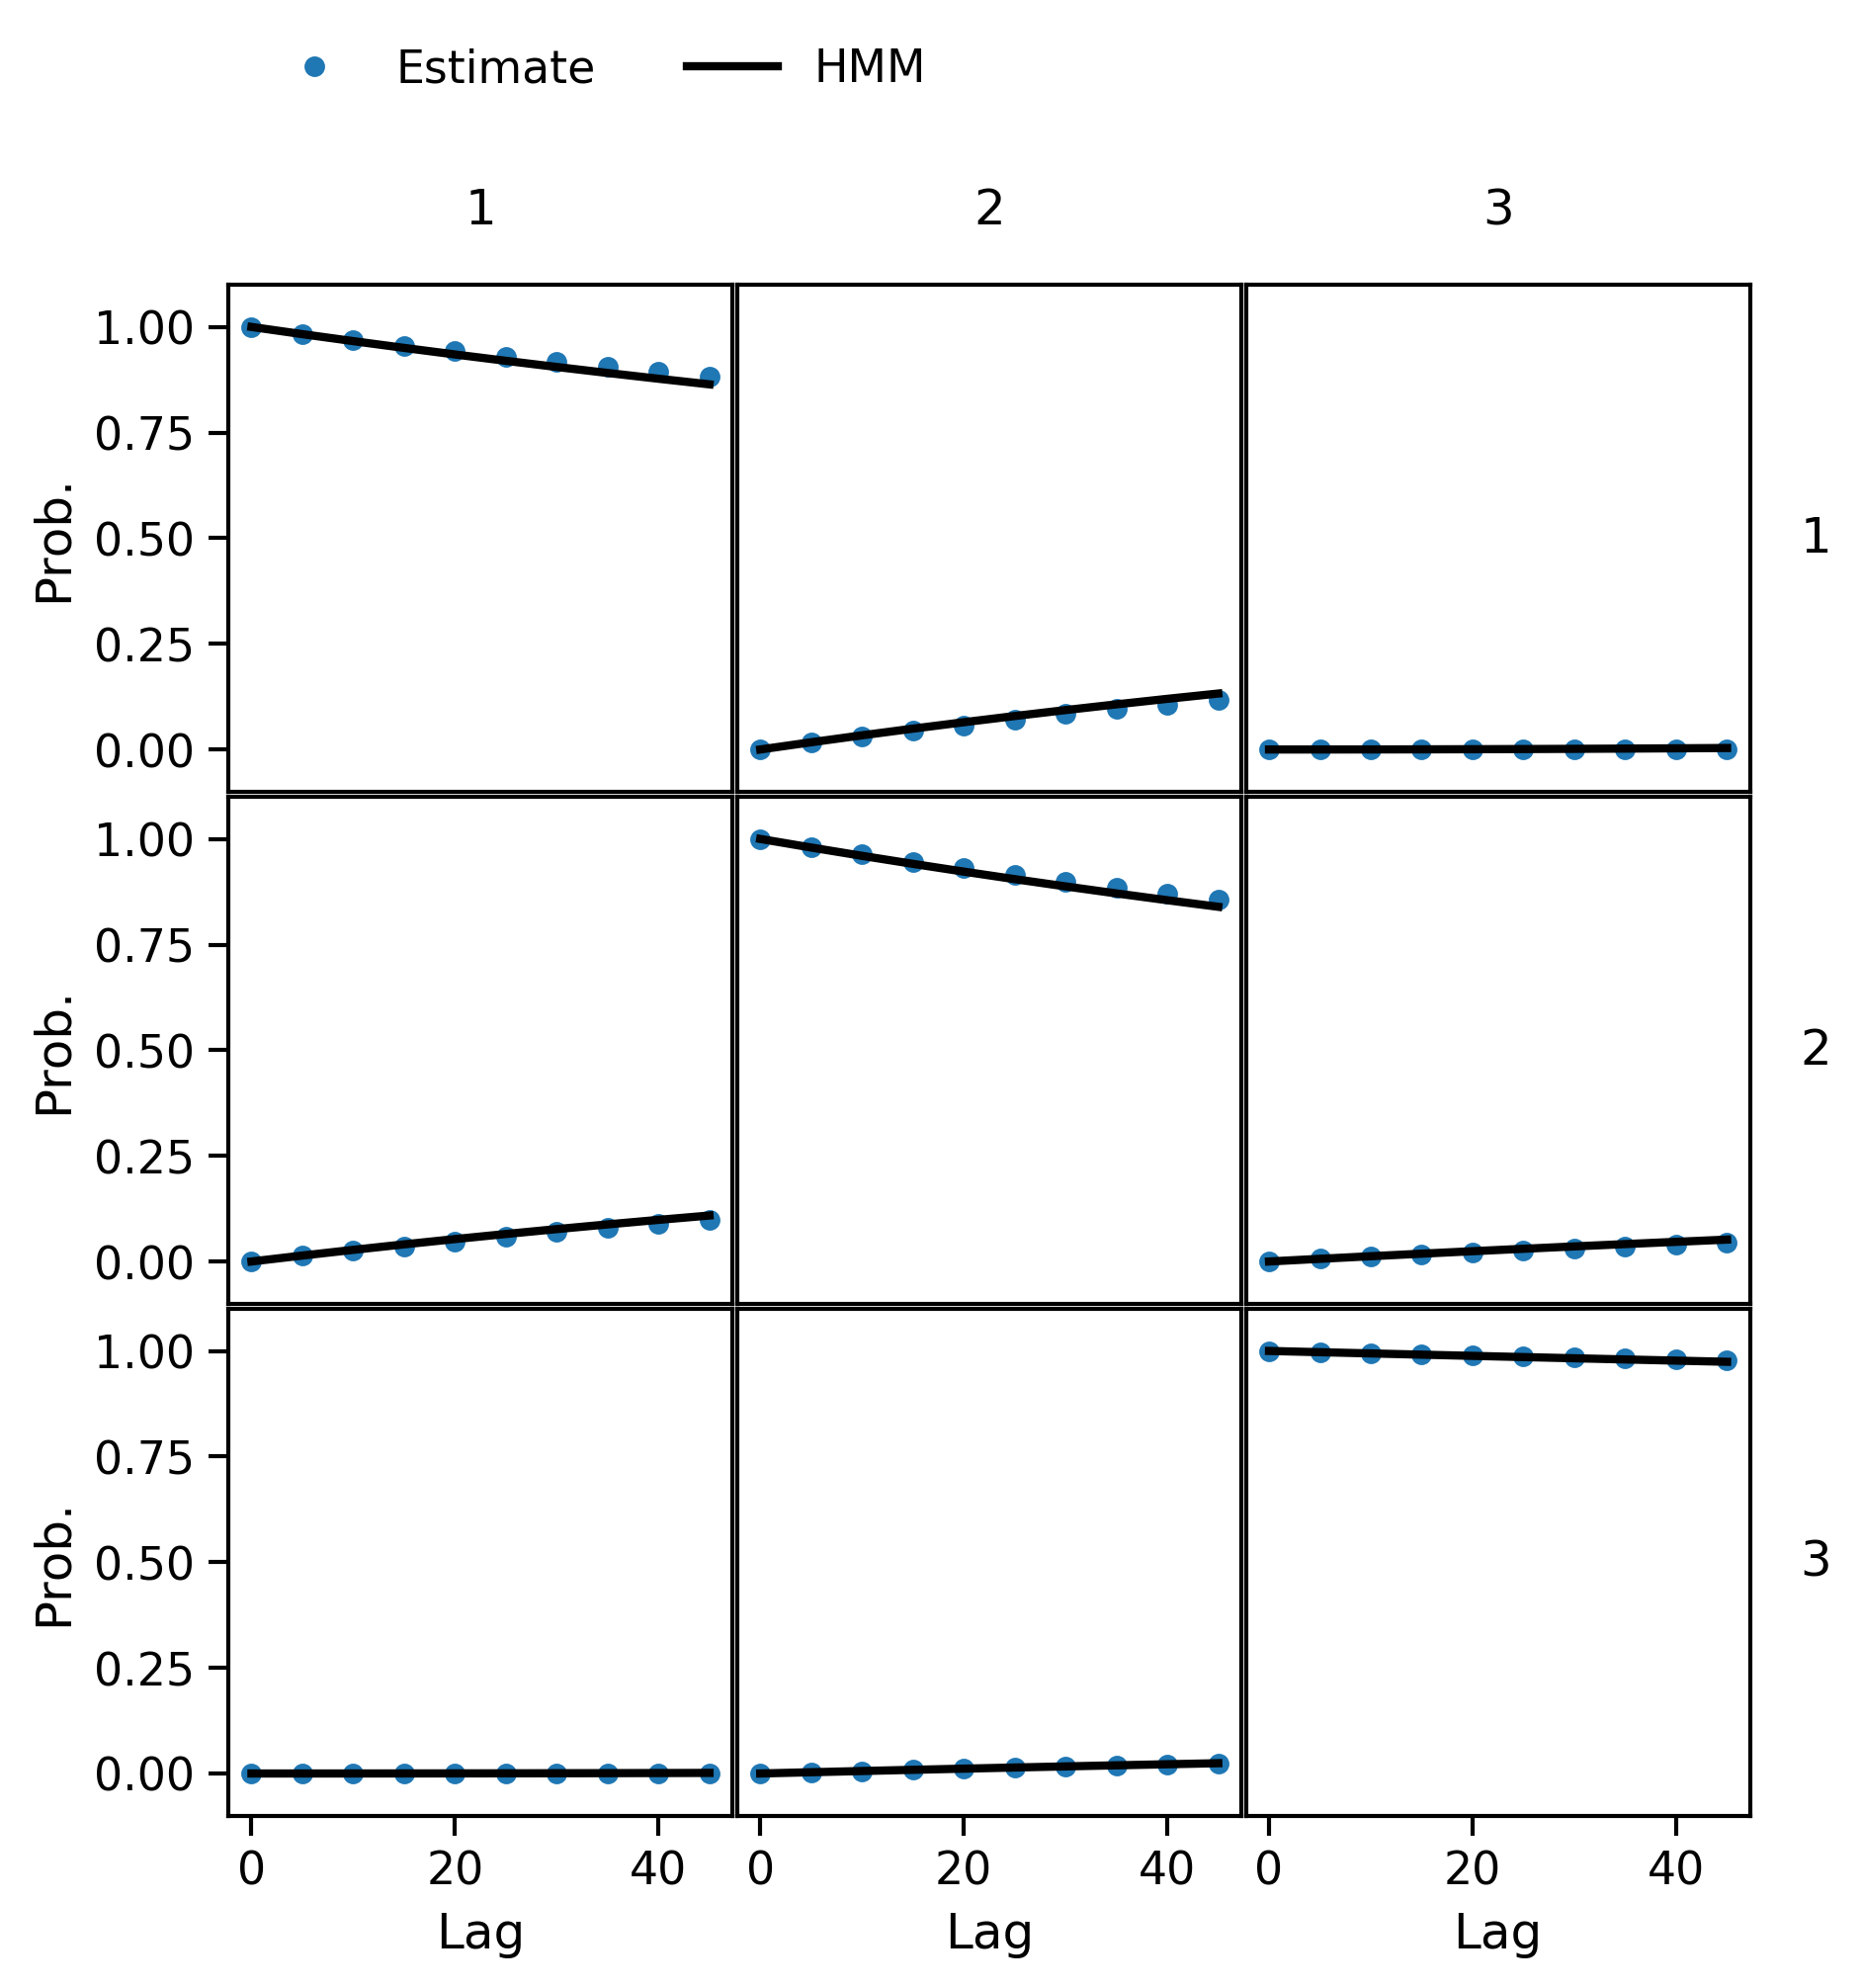
\includegraphics[width=0.4\textwidth]{chapters/hmm_selection/figures/ck_test_5_3.png}}
% \end{figure}

\begin{figure}
    \centering
    \mycaption{CK test for Prinz Potential with $\tau=5$ and $g=2$}
    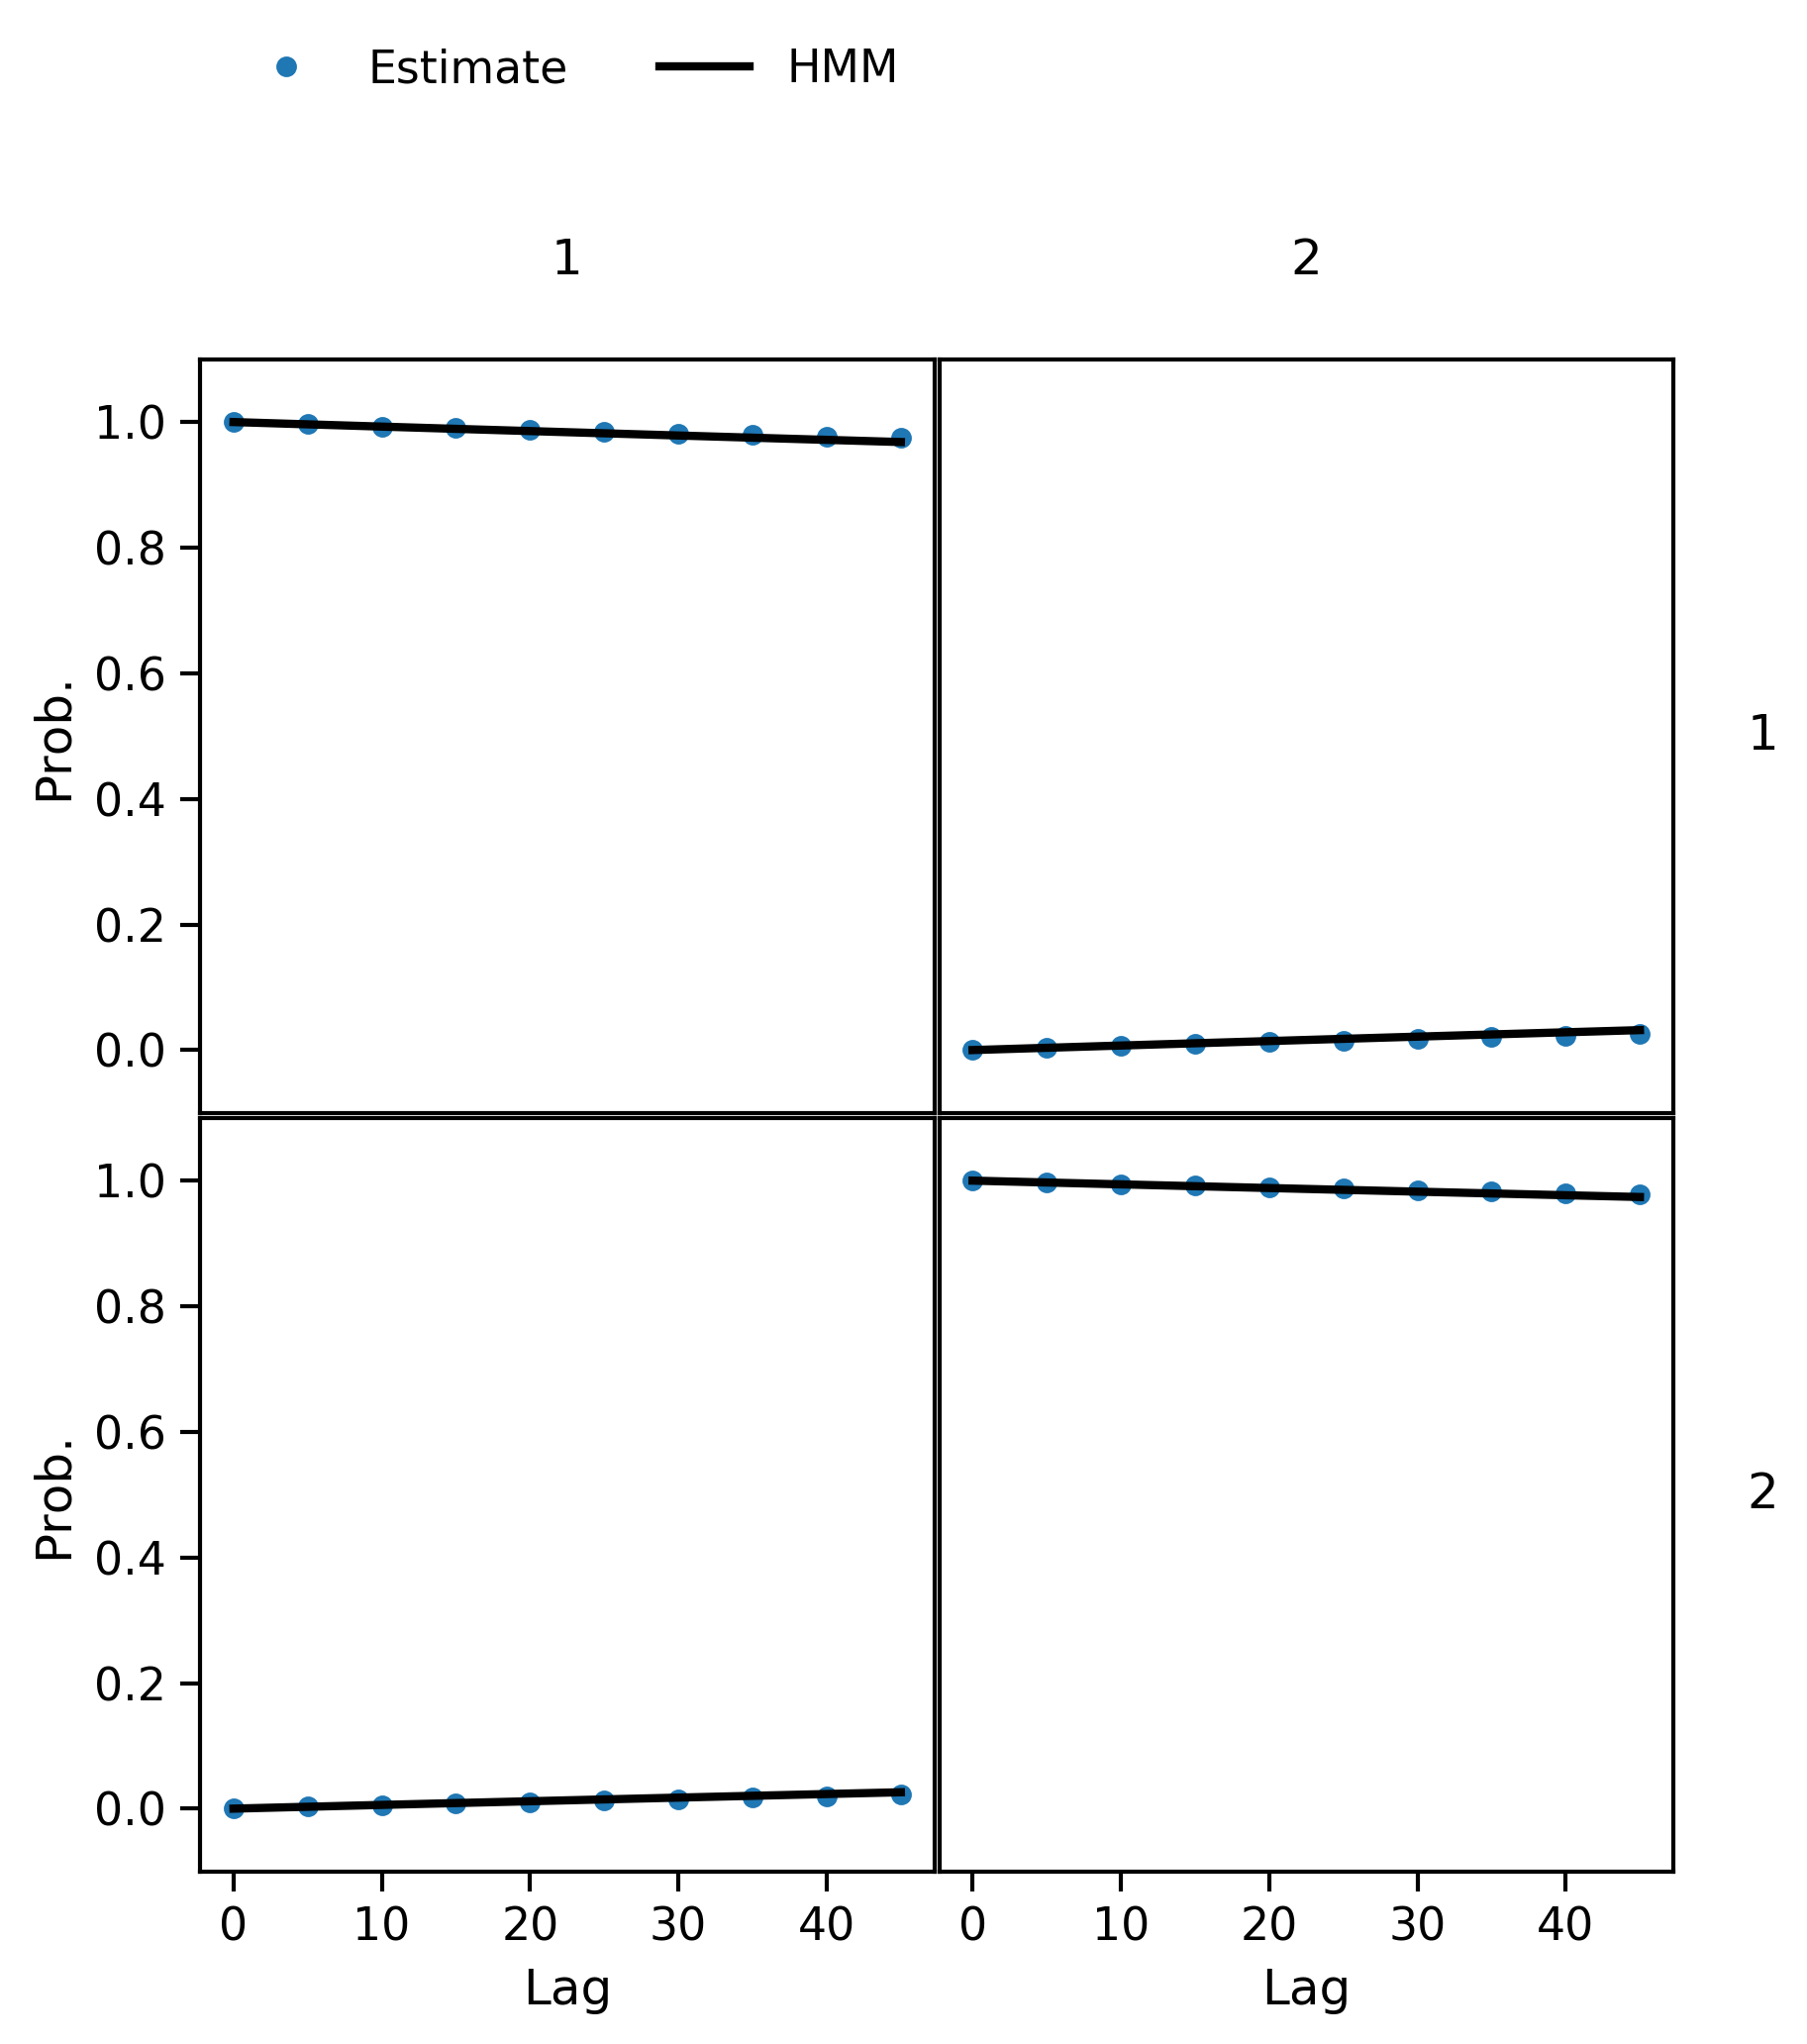
\includegraphics{chapters/hmm_selection/figures/ck_test_5_2.png}
    
    \label{fig:prinz_ck_test_5_2}
\end{figure}


\begin{figure}
    \centering
    \mycaption{CK test for Prinz Potential with $\tau=5$ and $g=3$}
    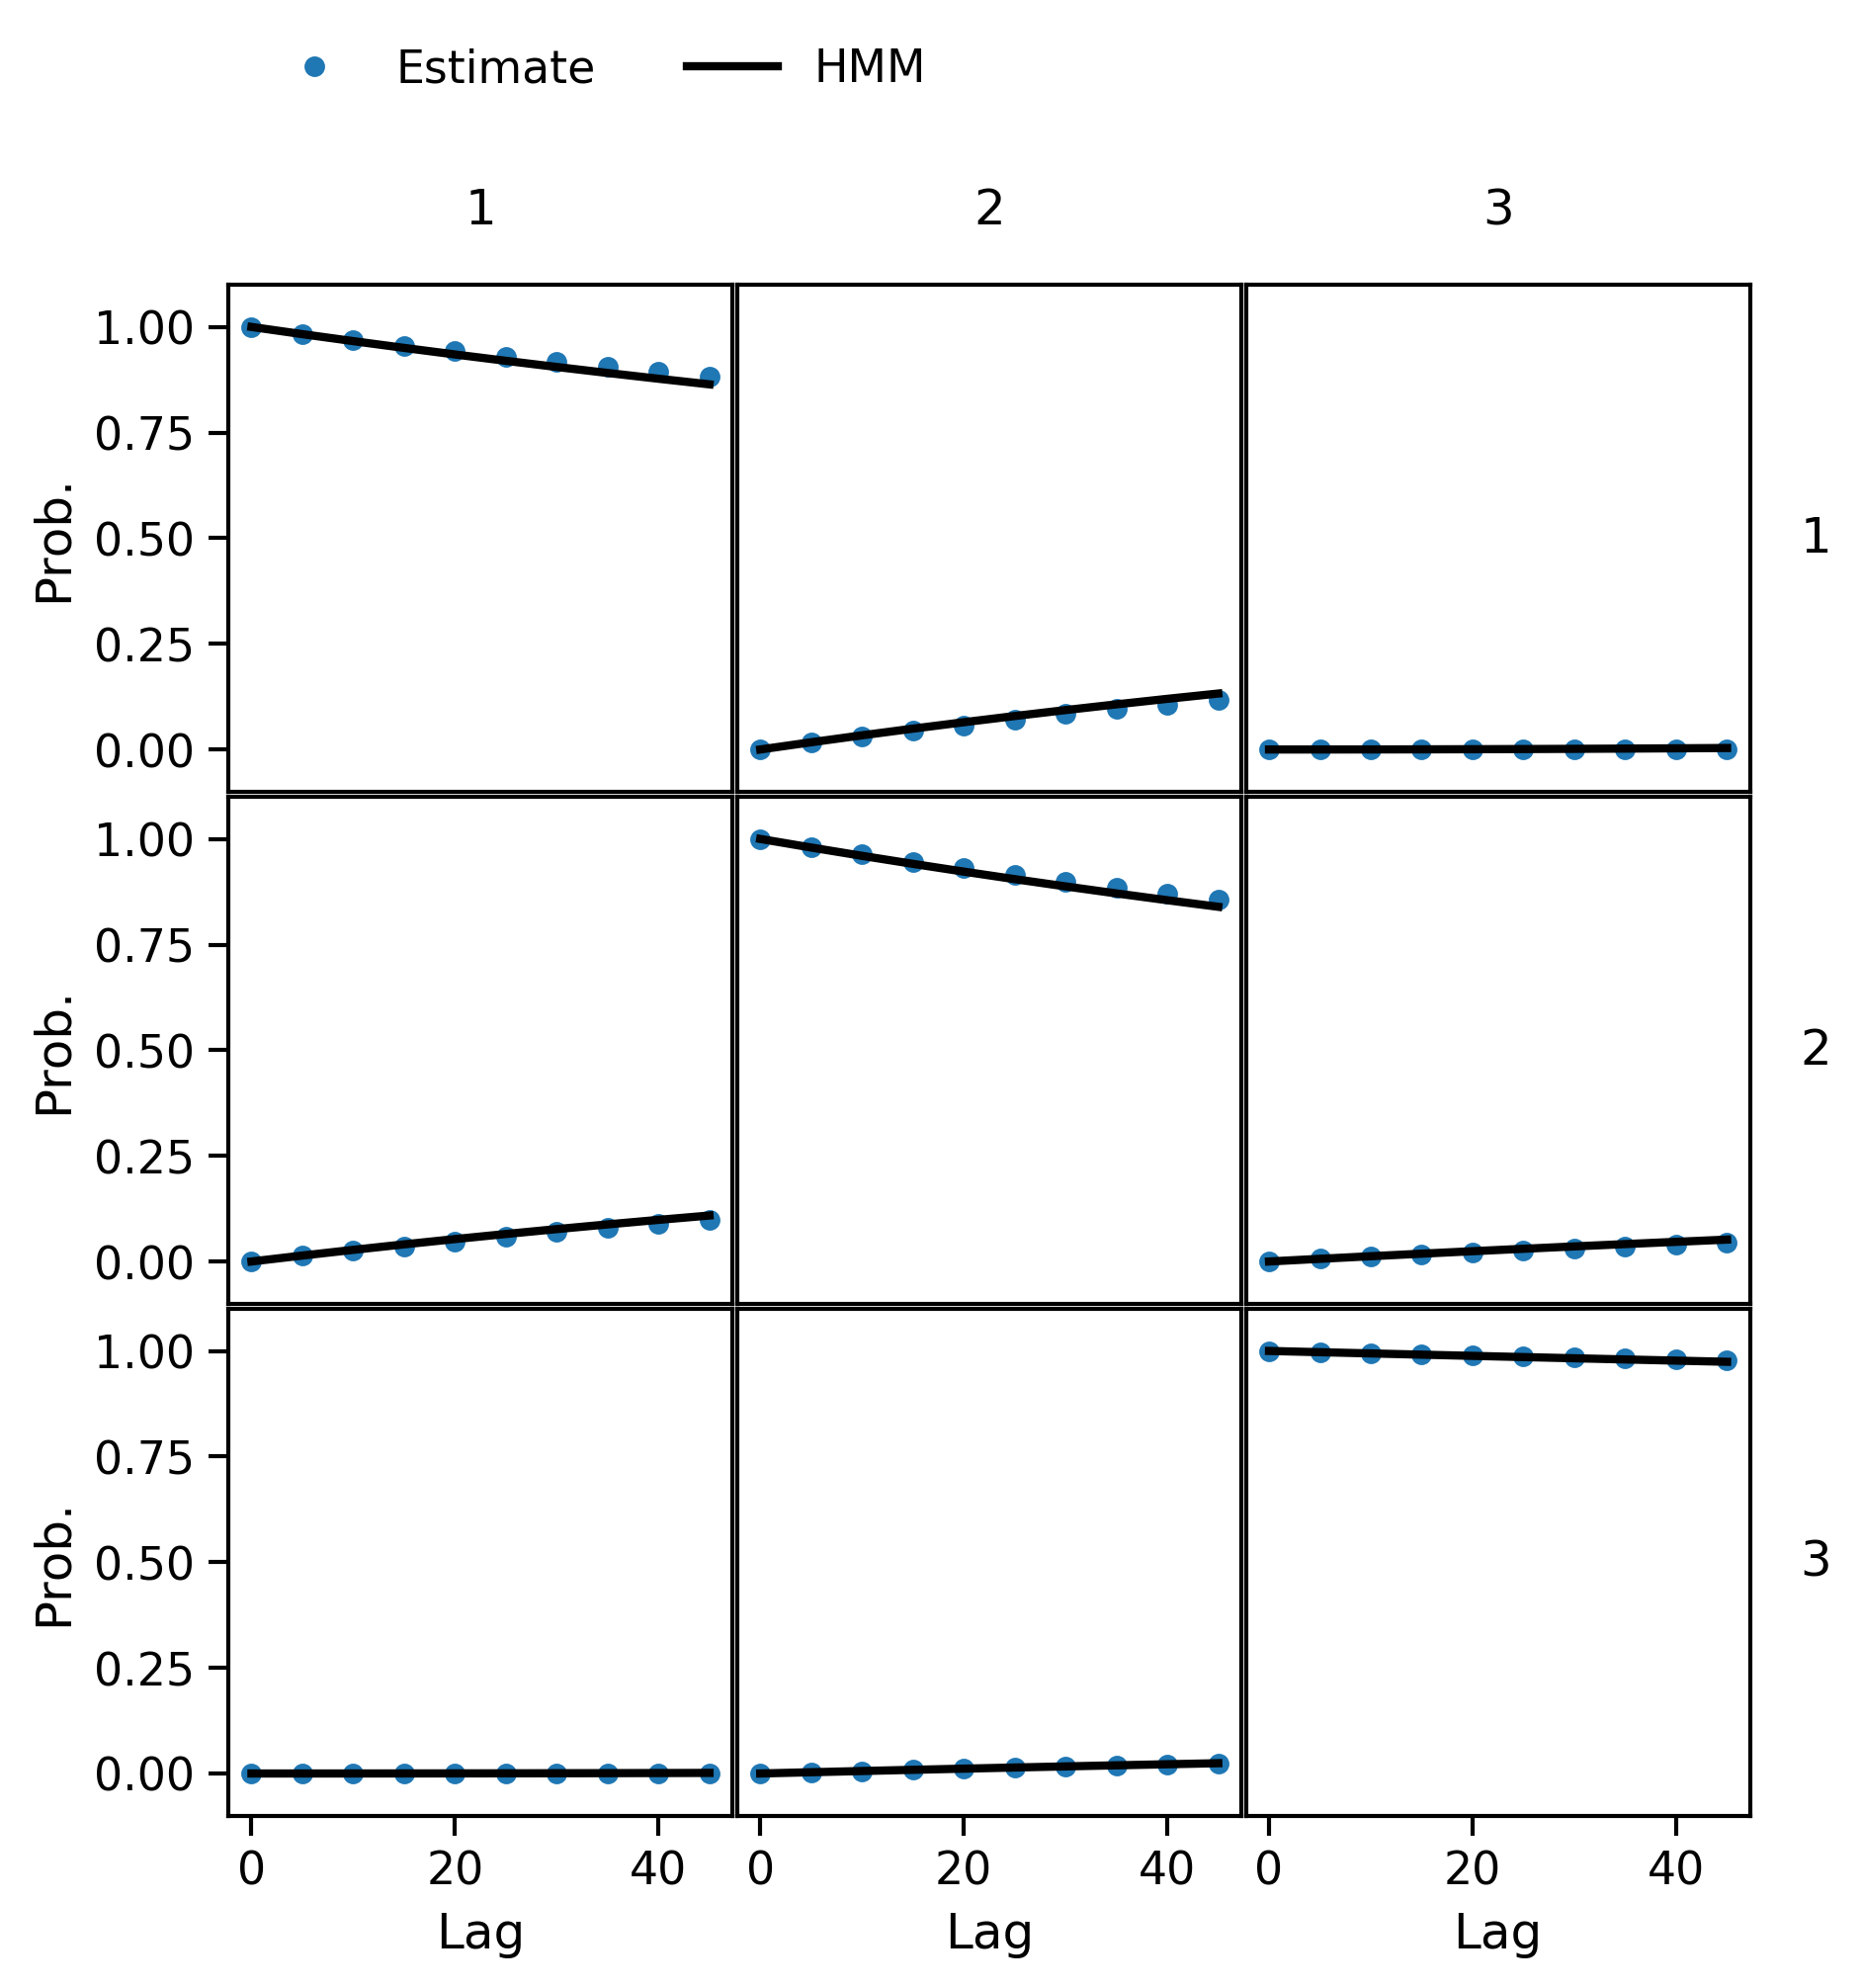
\includegraphics{chapters/hmm_selection/figures/ck_test_5_3.png}
    
    \label{fig:prinz_ck_test_5_3}
\end{figure}

\begin{figure}
    \centering
    \mycaption{CK test for Prinz Potential with $\tau=5$ and $g=4$}
    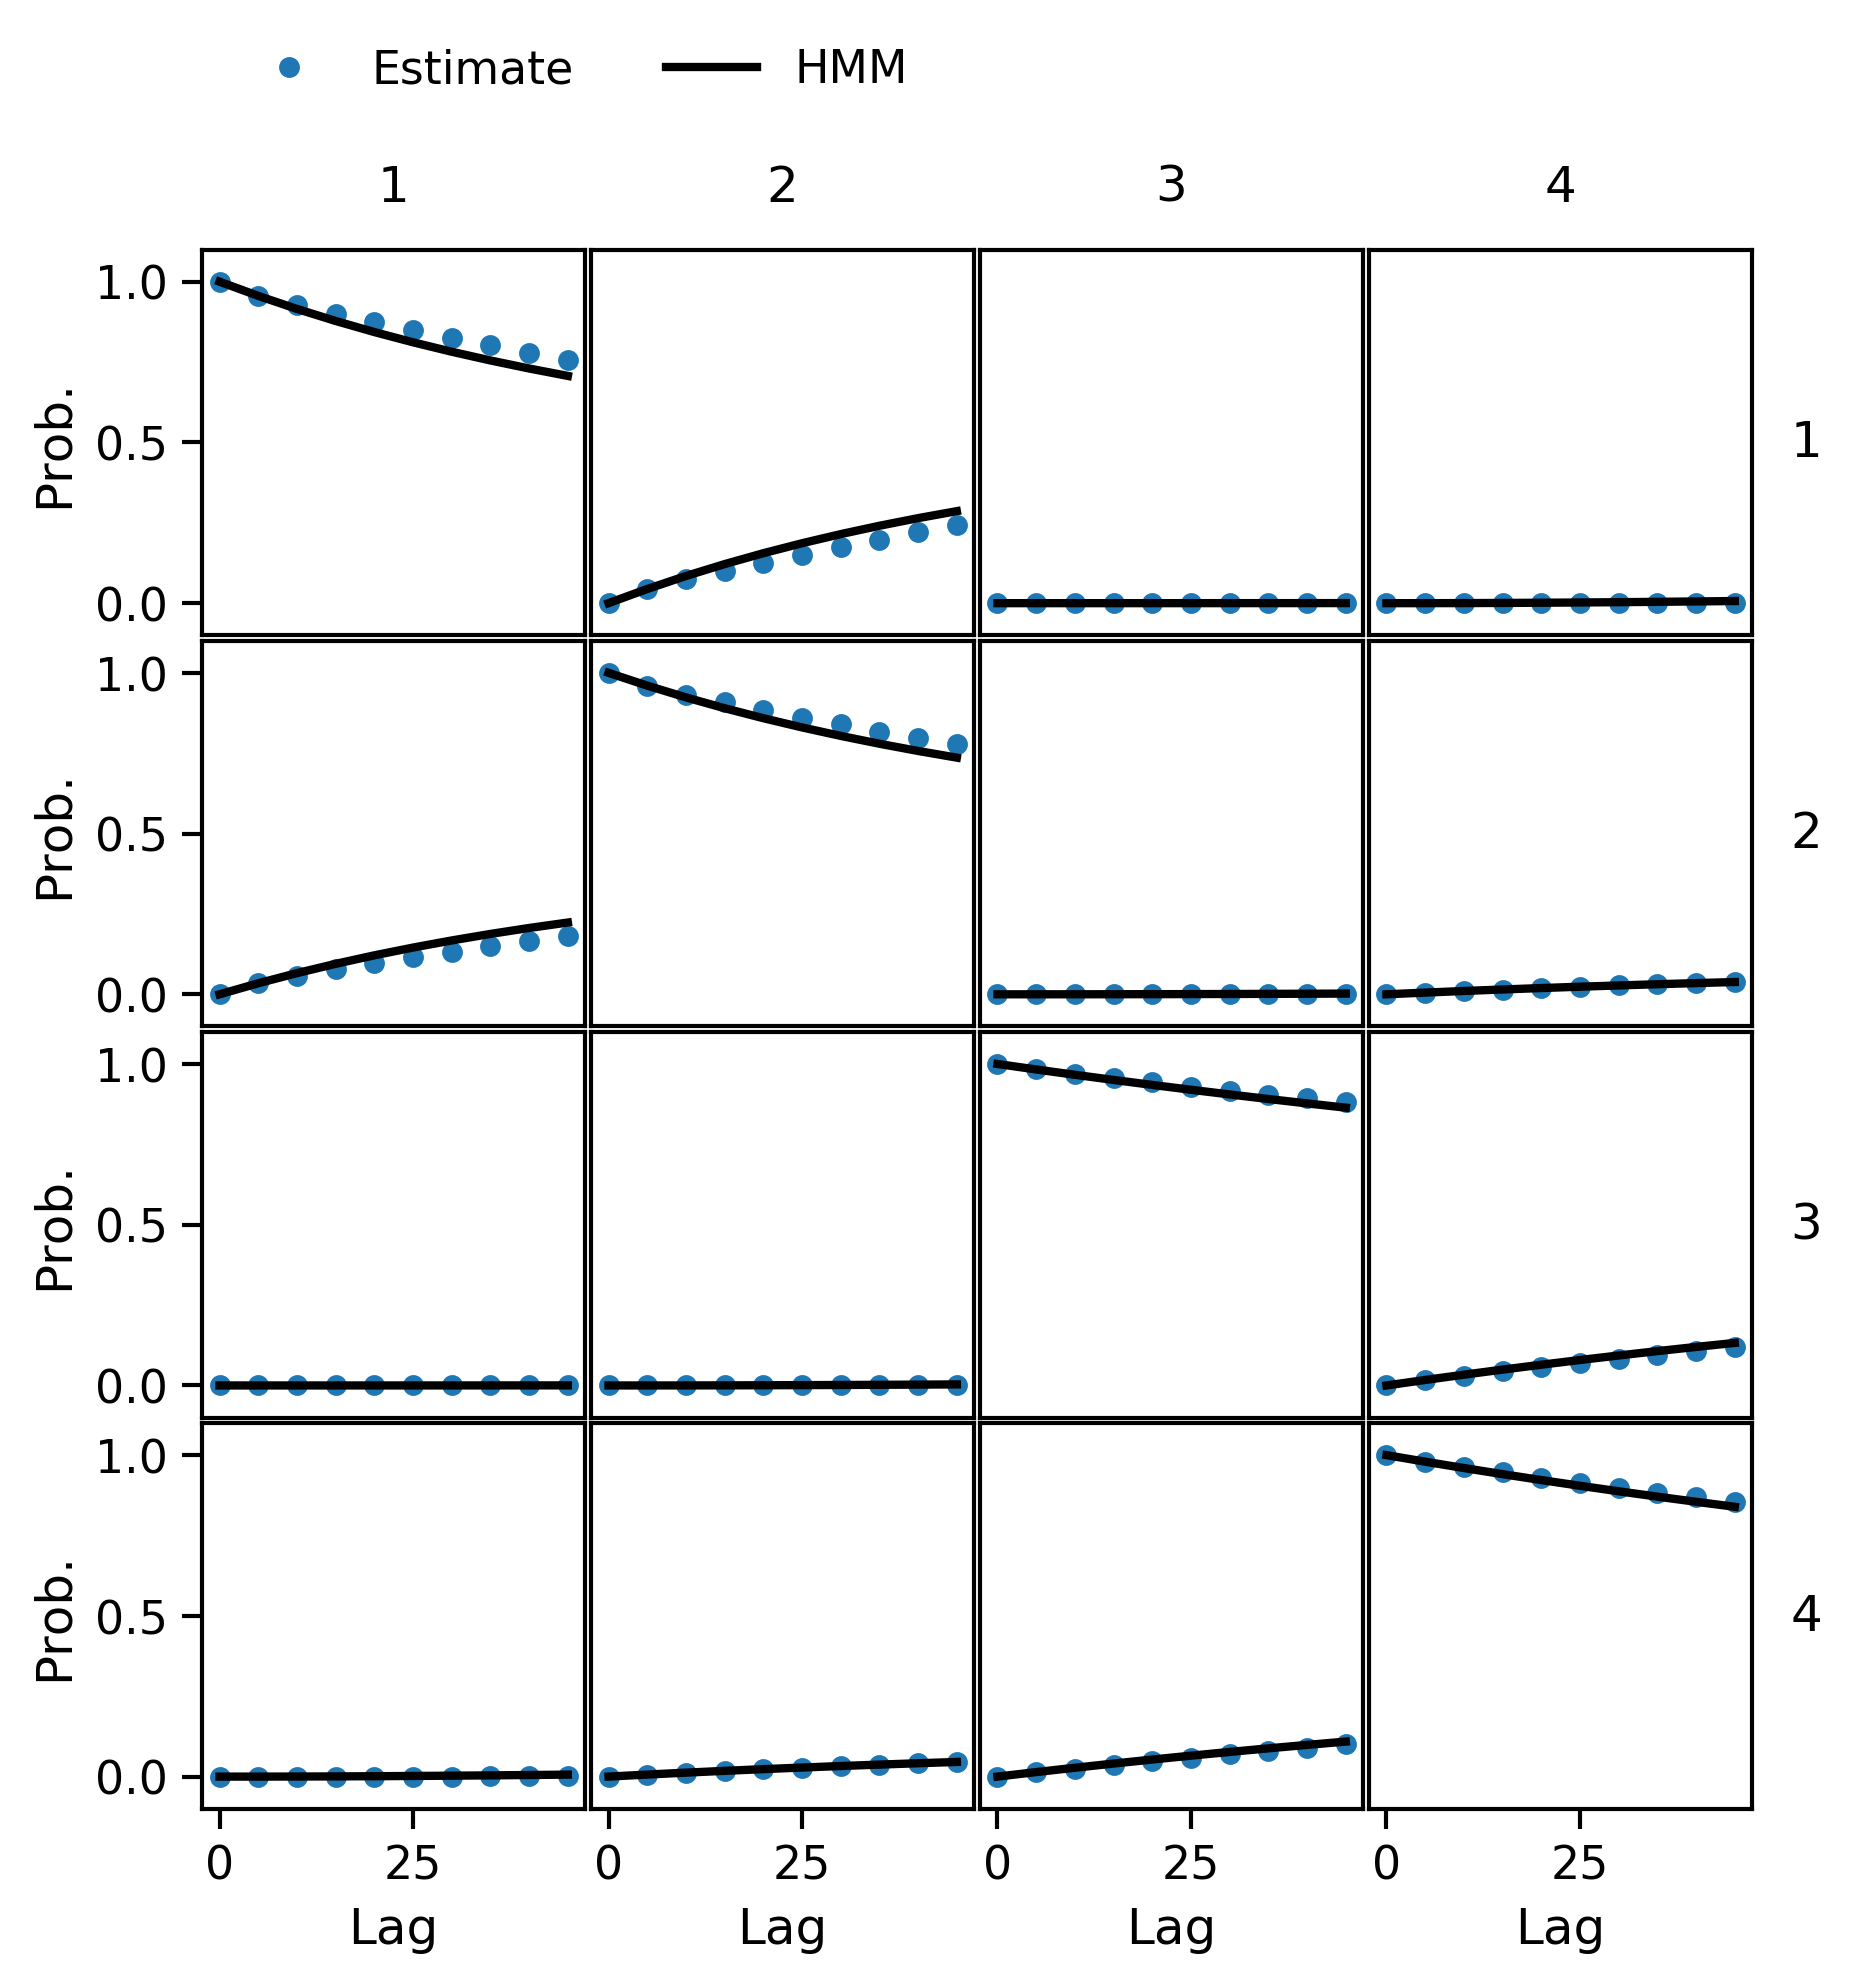
\includegraphics{chapters/hmm_selection/figures/ck_test_5_4.png}
    
    \label{fig:prinz_ck_test_5_4}
\end{figure}

\begin{figure}
    \centering
    \mycaption{CK test for Prinz Potential with $\tau=5$ and $g=5$}
    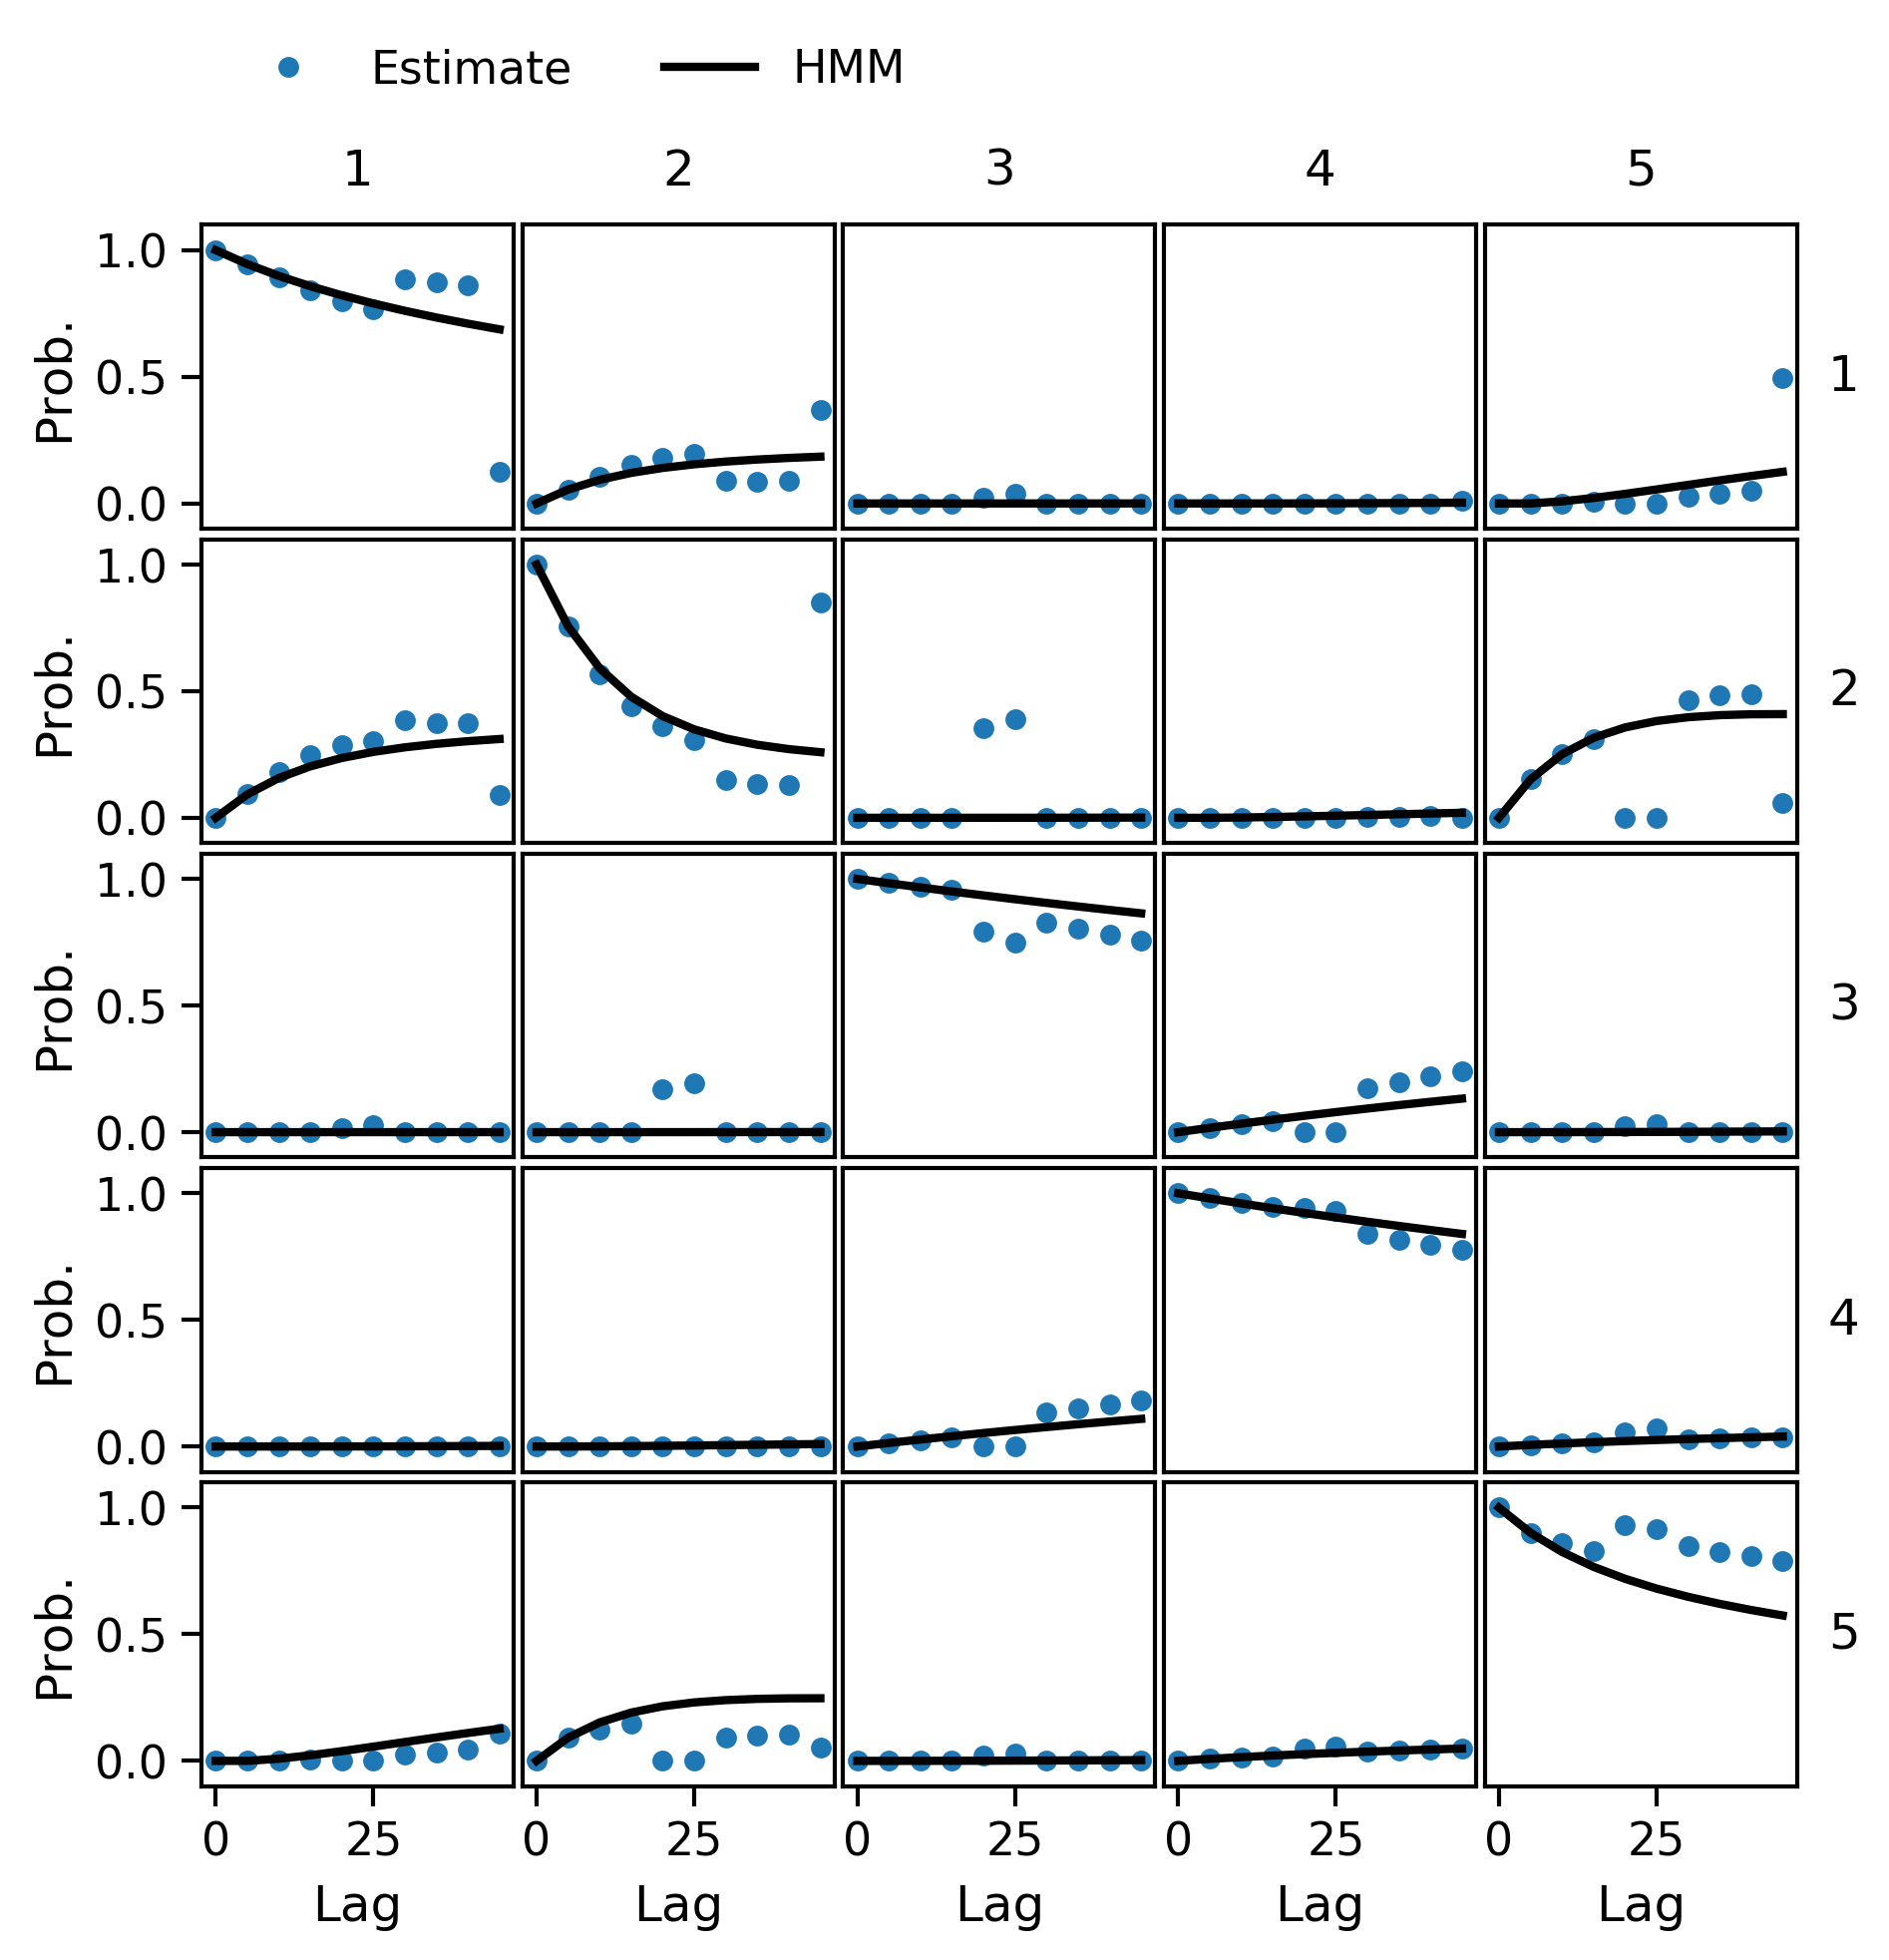
\includegraphics{chapters/hmm_selection/figures/ck_test_5_5.png}
    
    \label{fig:prinz_ck_test_5_5}
\end{figure}

\begin{figure}
    \centering
    \mycaption{CK test for Prinz Potential with $\tau=5$ and $g=9$}
    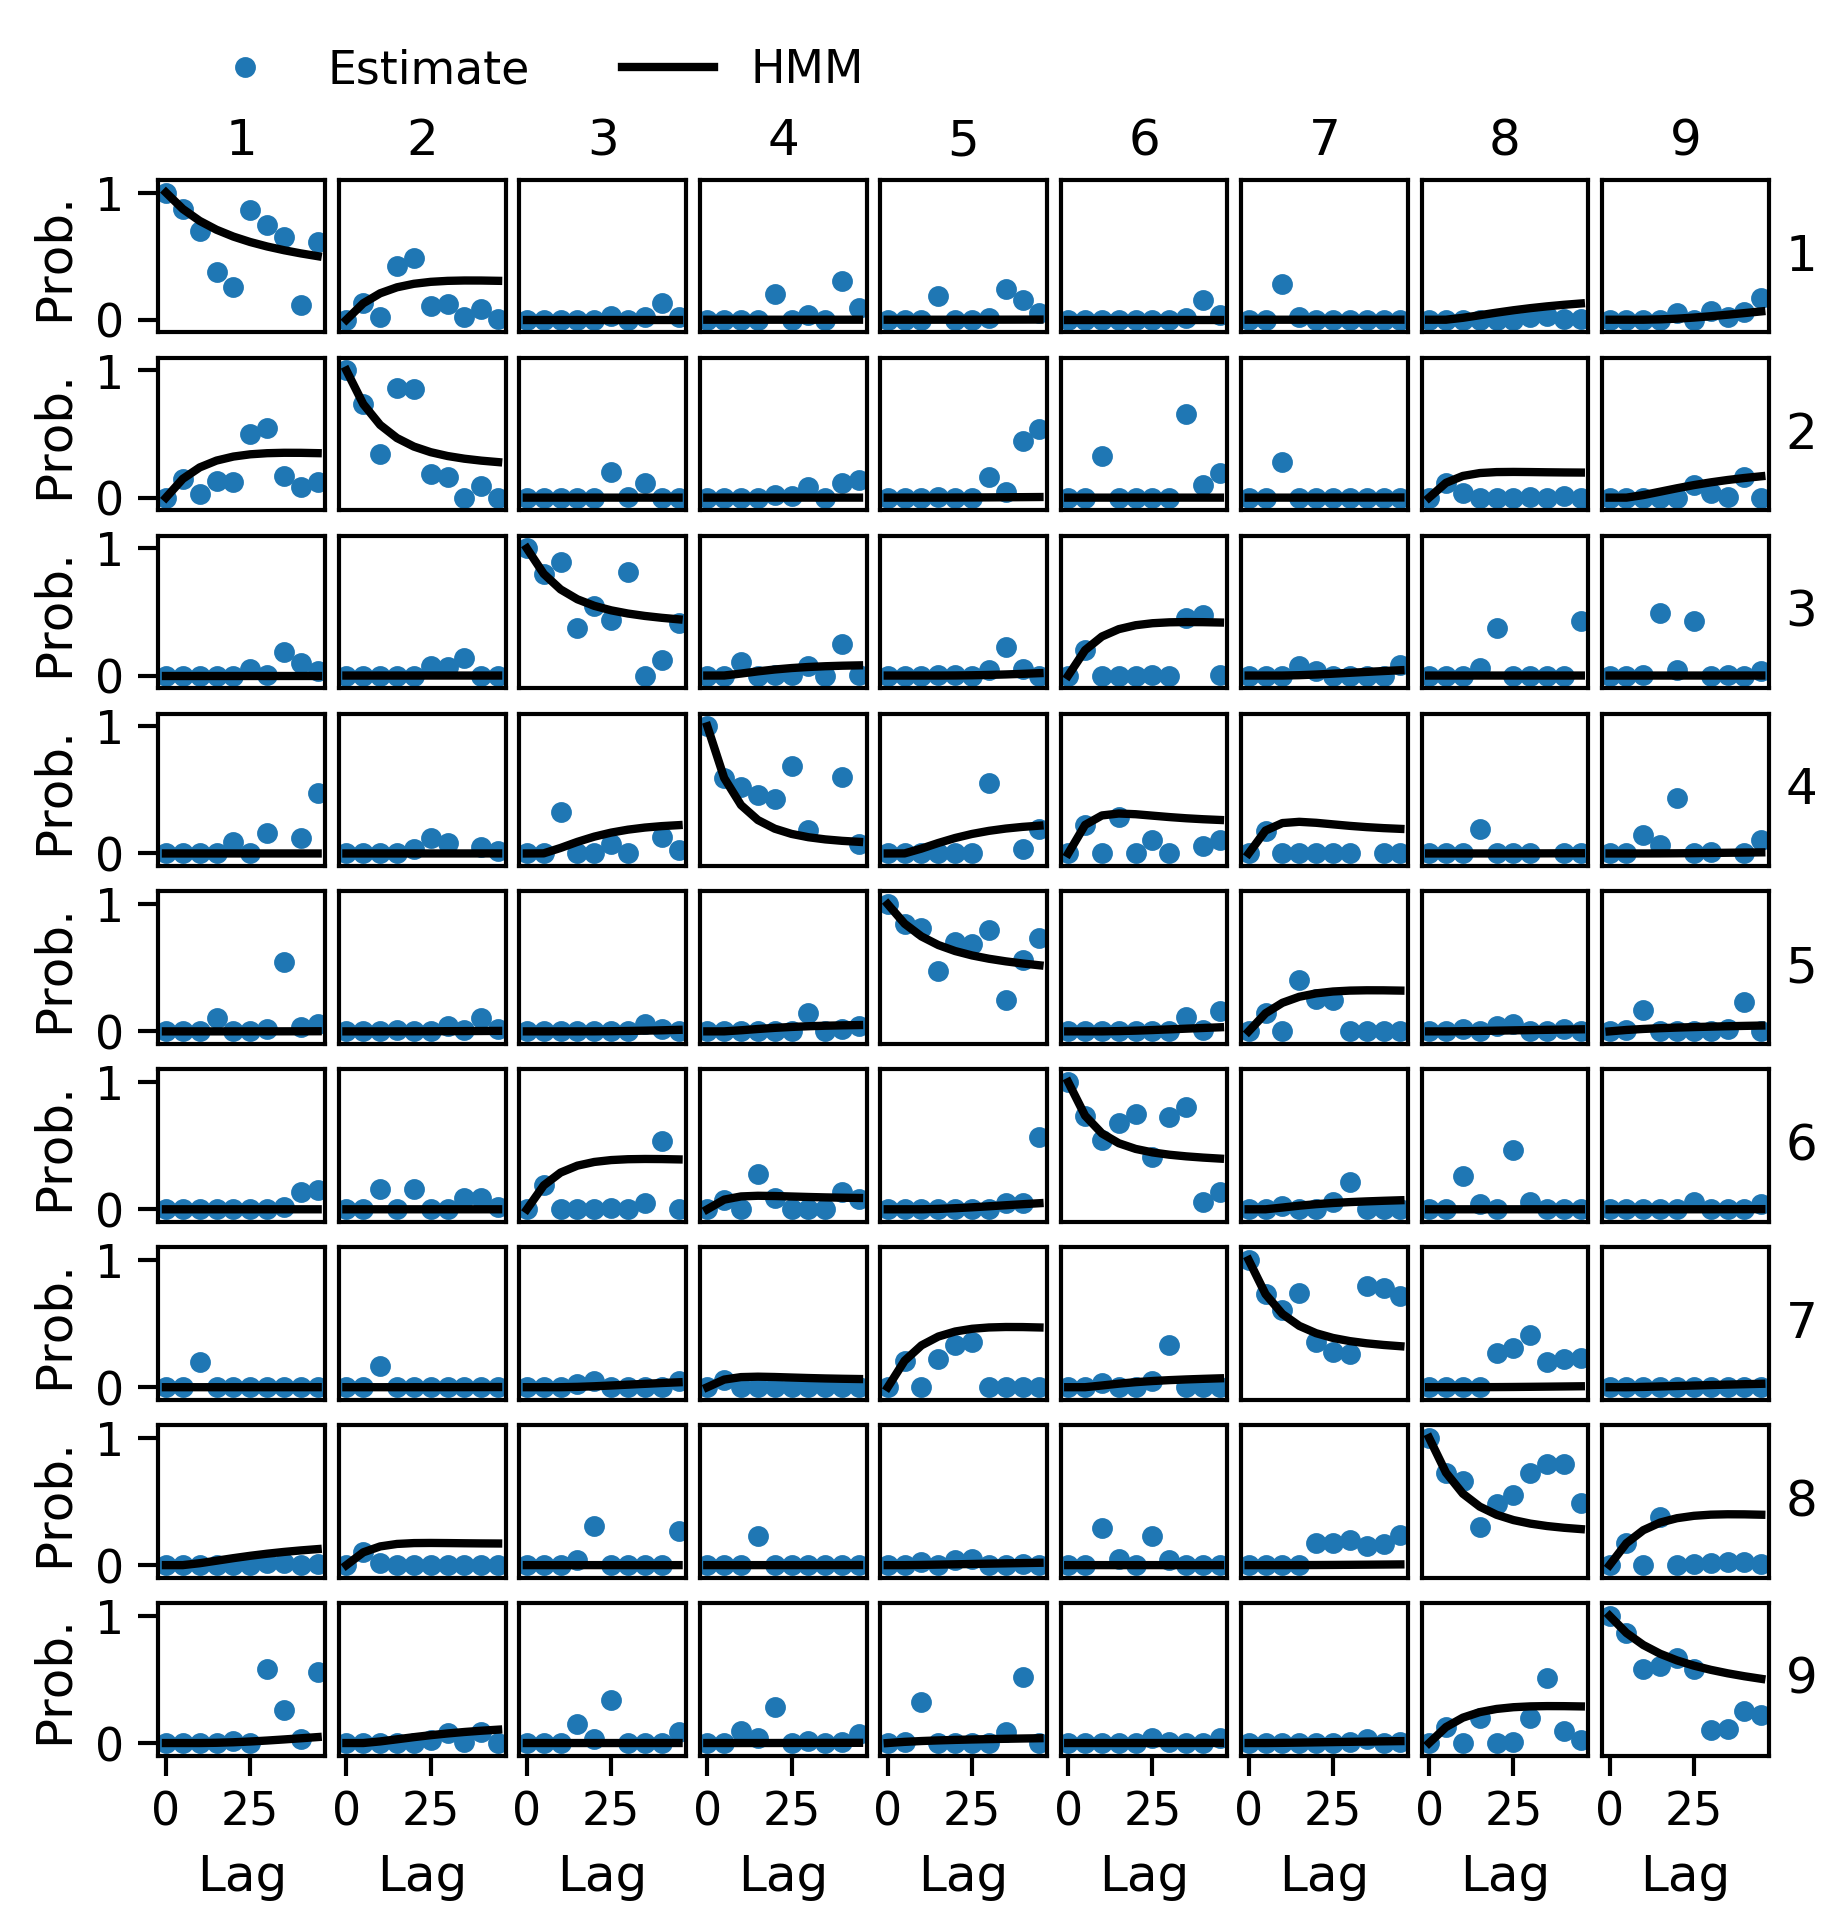
\includegraphics{chapters/hmm_selection/figures/ck_test_5_9.png}
    
    \label{fig:prinz_ck_test_5_9}
\end{figure}

\begin{figure}
    \centering
    \mycaption{CK test for Prinz Potential with $\tau=5$ and $g=10$}
    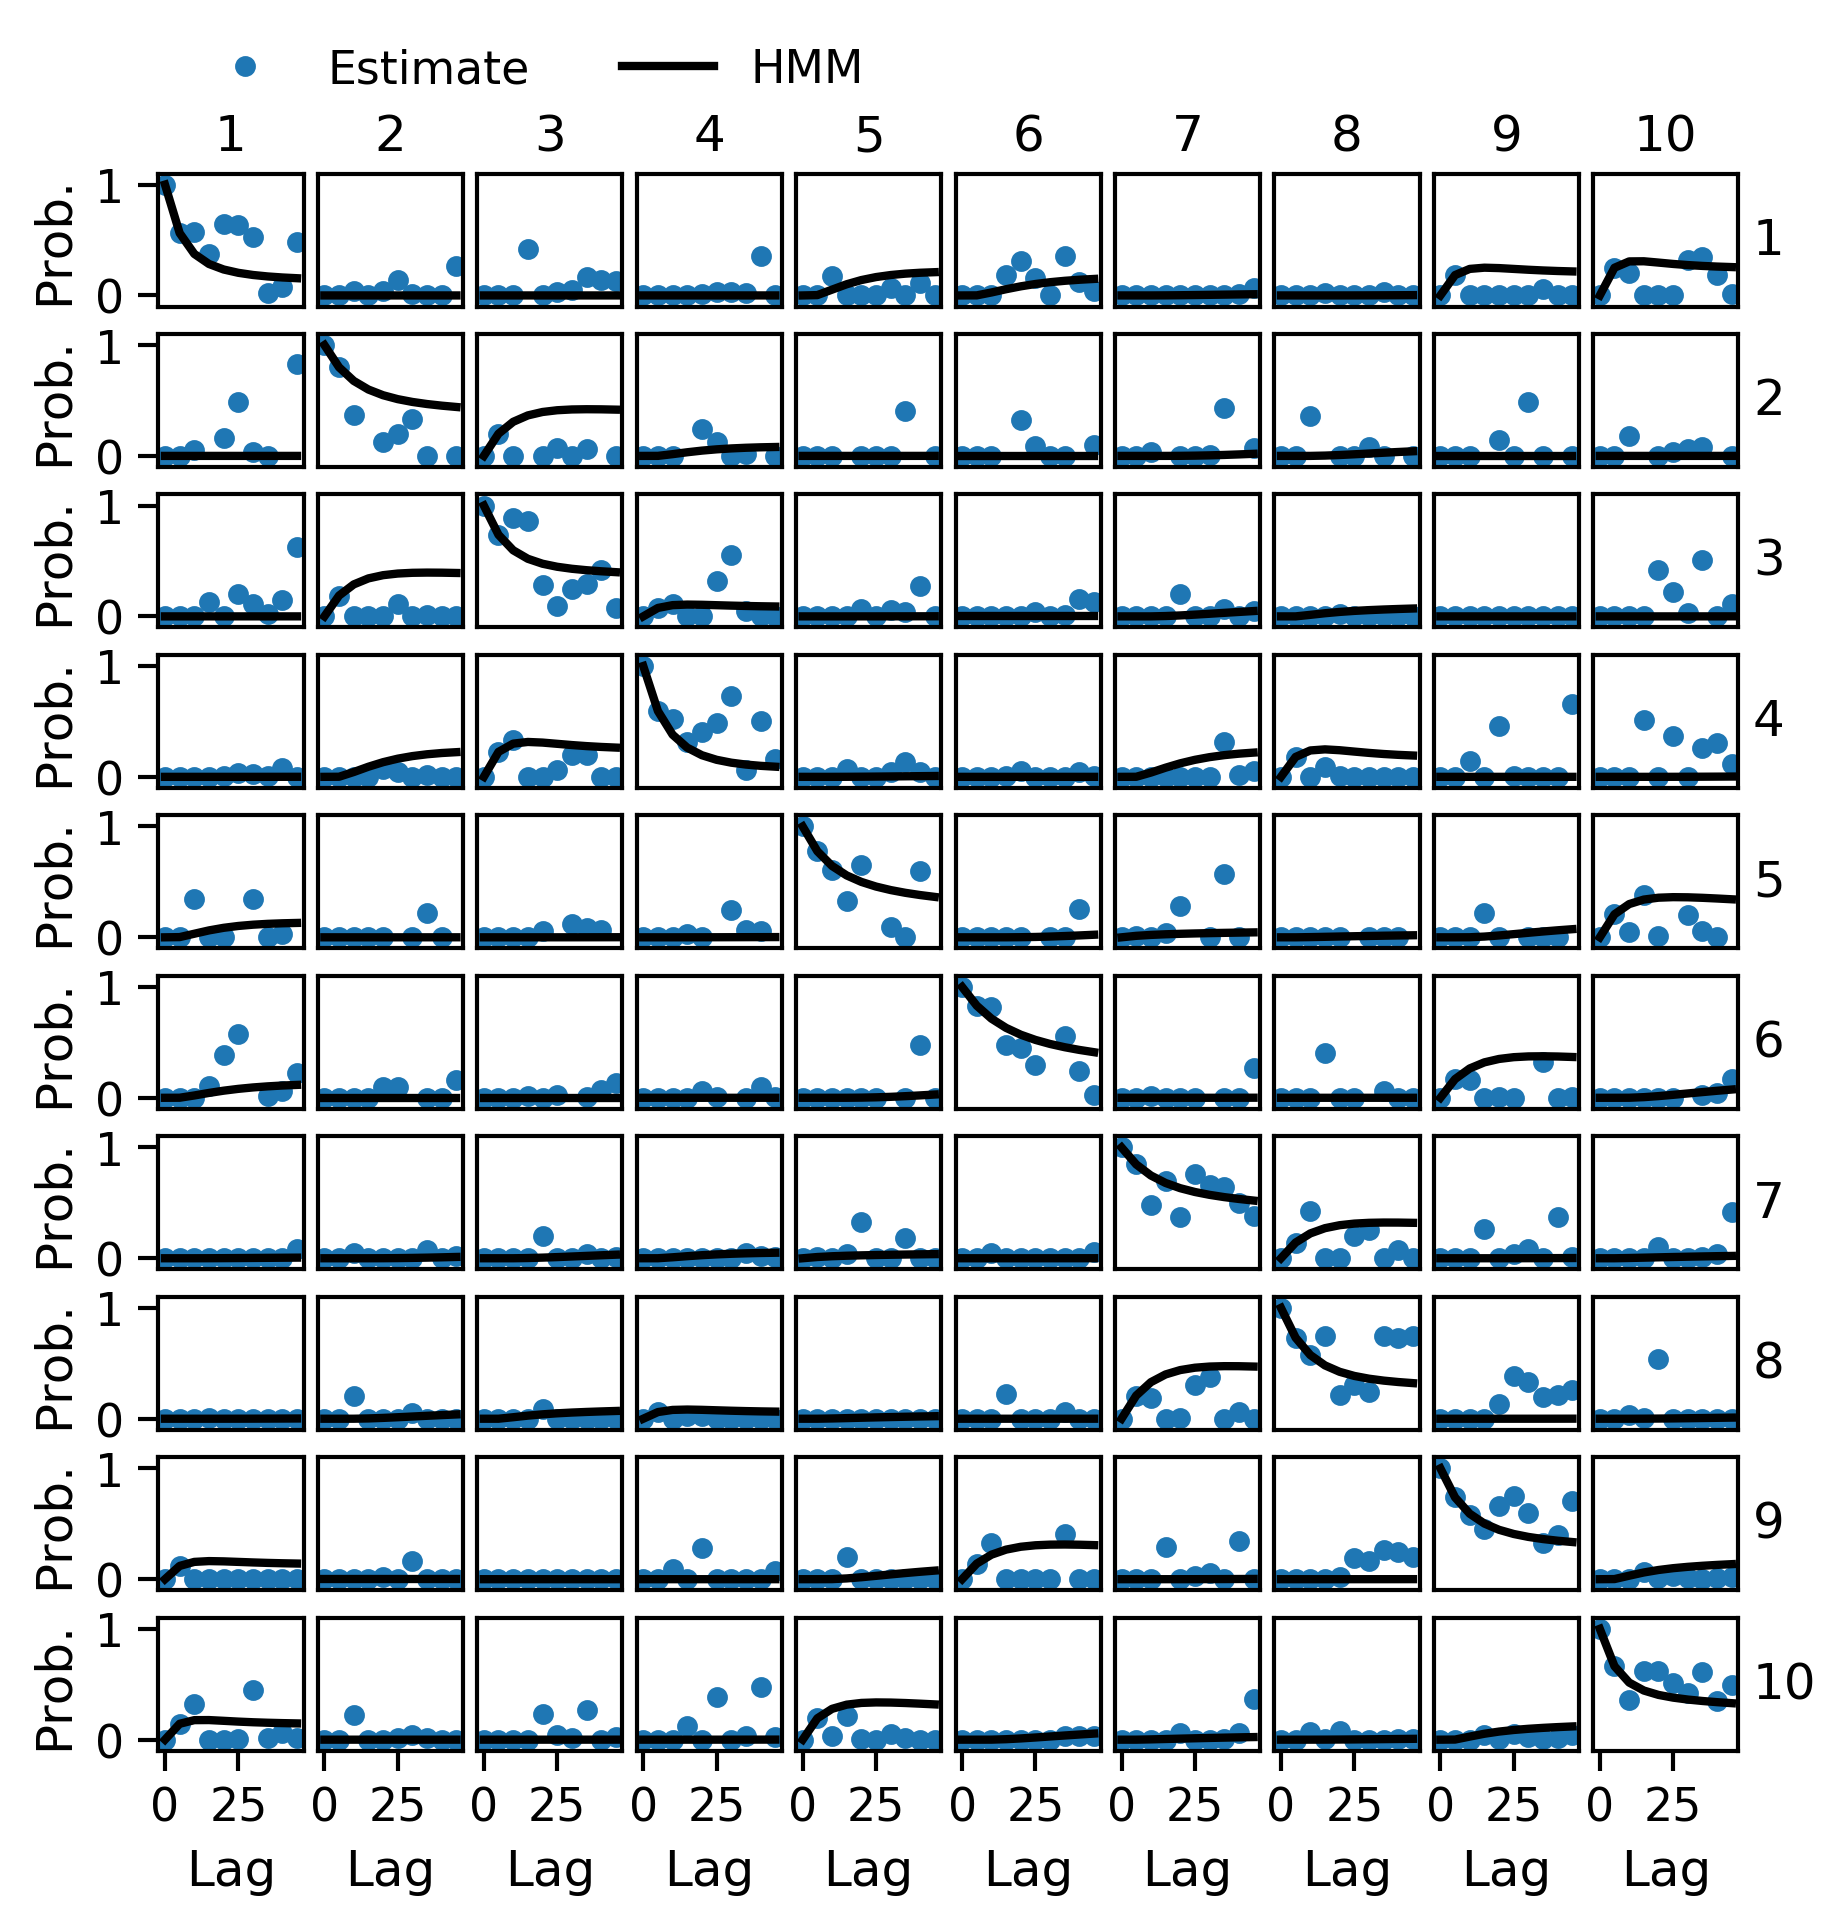
\includegraphics{chapters/hmm_selection/figures/ck_test_5_10.png}
    \label{fig:prinz_ck_test_5_10}
\end{figure}

\begin{figure}
    \centering
    \mycaption{implied timescales for $g = 2, 3, 4, 5, 9, 10$}
    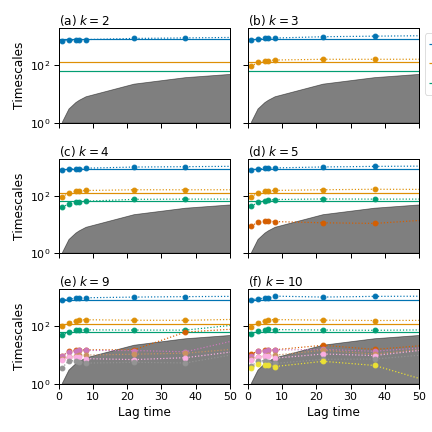
\includegraphics{chapters/hmm_selection/figures/its_tau_5.png}
    \label{fig:prinz_its_tau_5}
\end{figure}